% LaTeX thesis template.
% Version 1.6
%
% Department of Computer Science IV,
% University of Mannheim,
% Germany
%
% Based on the KOMA script classes.
% Created by Philip Mildner 2013-2015.
% If you have any feedback or if you find errors contact me:
% mildner@informatik.uni-mannheim.de
%
% Relevant class options:
%
% oneside:
% For shorter thesis like seminar papers you can use the single-sided layout, for longer thesis
% the double-sided layout is preferred (and it uses less paper, too). If you would like to have
% a single-sided print, use the 'oneside' option in the documentclass.
%
% BCOR=<value>:
% Depending on your method of binding, you might want to change the BCOR setting to account for
% the part of the pages that are hidden in the cover (e.g., set 'BCOR=10mm' if 1cm is hidden). 
%
% german:
% The standard behavior of this template is to produce English documents. If you would like to
% write your work in German, just include the 'german' option.
%
% draft:
% If you set the 'draft' option, overfull boxes will be highlighted in the PDF file so that you can
% find them more easily.
\documentclass[oneside]{pi4-thesis}

% The title page in this template has a pretty standard layout. While all relevant information are
% displayed on it, it surely could be improved to look nicer. You are invited to change the title
% page to your needs. If you have found a pleasing layout, I will be glad if you share it with me.
%
% Fill in the relevant information in the following lines.
%
% Choose between bachelor thesis or master thesis (or translate it to German).
\piivsubject{Bachelor Thesis\\
\vspace{5mm}
\includegraphics*{src/images/logo}
    }

% The title of your work.
\piivtitle{Business Information Visualization of time-oriented data: A comparison of current visualization-tools}
% Your name.
\piivauthor{Alena Beyer}
% Name of your supervisor.
\piivsupervisor{Prof. Dr.-Ing. Bernhard Preim}
% The date you submit your thesis. You can substitute the command with any date.
\date{\today}

% If you want to use the glossary make sure your 'makeindex' toolchain is working correctly.
% Alternetively, you might want to look into the 'xindy' option of the glossaries package.
\makeglossaries
\setcitestyle{square}

\begin{document}
% -----------------------------------------------------------------------------
% Acronyms Begin
\newacronym{hdr}{HDR}{High Dynamic Range}

\newacronym{ctan}{CTAN}{The Comprehensive \TeX{} Archive Network}

\newacronym{fim}{FIM}{Fachschaft für Mathematik und Informatik}
% Acronyms End
% -----------------------------------------------------------------------------
% -----------------------------------------------------------------------------
% Main Glossary Begin
\newglossaryentry{BIV}
 {
   name=BIV,
   description={Business Information Visualization}
}
% Main Glossary End
% -----------------------------------------------------------------------------

% Abstract is optional. If you do not use an abstract, remove it.
% ---------------------------------
% Begin of abstract
\abstractchap
% \blindtext creates a paragraph of non-sense text. Replace it with your actual content.
\blindtext
% End of abstract
% ---------------------------------

% ---------------------------------
% Begin of listings
\microtypesetup{protrusion=false} % disables protrusion locally in the document
\tableofcontents
% If you should not have any figures, tables or acronyms in your paper remove the according list.
\listoffigures
\listoftables
% Uncomment the next line if you use listings in your document.
% \lstlistoflistings
\microtypesetup{protrusion=true} % enables protrusion

\printglossary[type=\acronymtype]
% End of listings
% ---------------------------------

% ---------------------------------
% Begin of main part
\mainmatter

\chapter{Introduction}
\label{chap:introduction}

\section{Motivation}
\todo{ersten Outline durch richtige Einleitung ersetzen}
In the era of Big Data huge amounts of data are a new challenge for data visualization techniques. Beside technical challenges such as fast filtering and aggregation on databases there is the need for displaying billions of database records on a limited screen with a usual screen size of 1600x1200px. As the aim of visualization is insight into data, data visualization must present data in a way so that the reader gains new information out of the depicted visualization. 
As more and more companies discover the value of the data and understand how they can use data to unlock hidden mysteries about their customers, internal processes, e.g. to predict the moment when the customer will pay the bill, or production planning, big business data must be visualized in a ways that it generates insights. According to PwC's Global Data and Analytics Survey 2016 30\% of german companies in the medical and descriptive sector use big data in decision making. %(http://www.pwc.com/us/en/advisory-services/data-possibilities/big-decision-survey.html) 
In the current research some solutions exist already to the question how to "squeeze a billion pixels in a limited display"\cite{Shneiderman2008}. 


\section{Research Question}
This is why the topic of this thesis is the question: "Business Information Visualization of time-oriented data: A comparison of current visualization-tools".
Time-oriented data is only one selected data type out of other data types in information visualization. With the advancing mobile technology and the use of sensors for analytics the analysis of time-oriented data becomes more and more important for business. Time-oriented data is a well studied research area in which literature for advanced visualizations is widely available. 


\section{Structure of Work}
To answer the research question we will identify why advanced visualization methods are needed for displaying time series big data compared to traditional ones.
In defining the difference between traditional and advanced visualization techniques, 
taking psychological results in the perception of "many points" on a screen into account, 
describing the limits of traditional visualization techniques for big data.
Next, we will collect different advanced visualization techniques which make it possible to display big data and reach the above mentioned goal of "Insights in Data". 

Looking at the requirements for the presented advanced visualizations in big data we will bild a criteria catalogue after which some selected tools are judged. The criteria catalogue should involve:\\*
Does the tool enables different kinds of advanced visualization types\\*
Allows the tool to implement techniques to realize the research findings about visualizations in big data? (e.g. Is it possible to aggregate visualizations?) \\*
For the test we will select some commercial and open source tools. The criteria to select the tools is not fixed yet. One possibility could be the marketshare and the diversity how the tools are unique compared to other tools.\\*
Last we will apply the criteria to the tools and come to a conclusion and answer to the question above.


\chapter{Definitions and Related Work}
\label{chap:concepts}
In this chapter we repeat basic concepts related to the topic of this thesis by defining them and providing an overview about the current literature. The order of definitions is not alphabetical - instead content-related definitions are grouped together. Related work can be summarized to the following research areas: business information visualization,  time-oriented data visualization, large scale visualization and surveys of visualization tools. 

\section{Definitions}
\textbf{Information Visualization} is the graphical representation of non-spatial or abstract data  \cite{Keim2006}. In contrast to scientific visualization, data information visualization does not have an inherent 2D or 3D structure  \cite{Shneiderman2008} and thus, no spatial relation. Abstract data usually exists in data tables with rows and columns. These columns are mapped in Information Visualization to graphical attributes such as position, color, size, orientation, texture or hue. 
Since business data is usually abstract, discrete and multivariate  \cite{Tegarden1999}, the type of visualization for business data is Information Visualization.
\par
\textbf{Data visualization} is a more general term for generating a graphical representation with data and is used in Business Intelligence (\gls{BI}), Analytics, data discovery and in visual analytics.
\par
\textbf{Business Information Visualization} (\gls{BIV}) \label{BIV} is defined as the use of visualization technologies to visualize business data  \cite{Tegarden1999}. While business data appears in multiple applications, \gls{BIV} is usually achieved with the help of computer tools - ranging from data loading to interactive visual analysis. Interactive visual analysis in businesses is often used to do self-service data science \cite{Russom2011,Parenteau2016,SAS2012,Curran2005}. \textbf{Self-Service} data visualization describes an approach that encourages a broad public to do data analysis with easy-to-use tools.
\par
\textbf{Advanced Data Visualization} (\gls{ADV}) in our understanding is a visualization technique which is able to scale to large and huge amounts of data.
\par
\textbf{Large Data}: To characterize the data volume we follow a definition of Huber. He divided data into small, medium, large, huge and massive data. Large data according to  \cite{Huber1994} is defined as data sets with $10^6$ and huge data with $10^8$ data entries. We are considering large and huge amounts of data.
\par
\textbf{Abstract data} is defined as data without any spatial relationship in the data  \cite{Shneiderman1996}. 
\par
\textbf{Discrete data} is data which can be mapped to integer values.
\par
\textbf{Multivariate data} is often mixed-up with the term multi-dimensional. For this reason we define  multivariate data by the number of dependent attributes. If the data set holds more than two dependent attributes then we call the data \textit{multivariate}. In contrast, multi-dimensional depicts the number of independent attributes of a data set \cite{Aigner2011}.
Multivariate time series are time series where one data item holds several variables at the same point of time \cite{Aigner2011}. In the analysis of multivariate time series of different variables and their combinations are interesting. In order to gain understanding of their development over time, the challenge of multivariate data is the selection of meaningful dimensions and their visualizations. 
\par
\textbf{Visual Scalability}\label{scalability} or "perceptual scalability" is defined as the capability of visualization tools to display large data sets in an effective manner  \cite{Eick2002}\label{effective}. In the context of time-oriented business data \textbf{effective} means the presentation of patterns to support the user tasks. To measure the visual scalability of different visualization techniques for time-oriented data we refer to the work of Eick  \cite{Eick2002}. He proposed to measure visual scalability by the database metrics of the data set and the visual characteristics of the visualization technique.
\par
\textbf{Database metrics}\label{databasemetrics} assess the size of the database in bytes, in rows or in columns \cite{Eick2002}. For multi-dimensional data, database metrics are a combination of the number of rows and columns.
\par
\textbf{Visualization characteristics} describe the number of elements and attributes presented on the screen and measure how many distinct items a visualization technique can display \cite{Eick2002}. This number is measured at the visualization technique level.
\par
\textbf{Visualization Tools}\label{tools} are computer tools and frameworks which offer a range of chart types to support visual data exploration. Tools for visual data exploration have different purposes which range from Business Intelligence (\gls{BI}) and Analytics, data discovery, data mining to visualization tools. Since the differentiation between those tools is not selective and the terms are not clearly distinguished we make the following differentiation:
Data mining tools cover the extraction of patterns and model the underlying data structure  \cite{FerreiradeOliveira2003}. Data mining is based on automated algorithms which detect relevant patterns and display the results in terms of statistical reports or visualizations. In contrast to automated analysis, \textbf{visual data exploration} (\gls{VDA}) is a human guided process  \cite{FerreiradeOliveira2003}. First, data is displayed on the screen as a visualization and with the help of human visual capabilities new hypotheses are formed. With visualization tools the user can interact with the data by changing parameters, filtering, zooming and defining new user input. Visualization tools can denote both tools to represent data mining results and tools for \gls{VDA}. We will use visualization tool in terms of a tool which supports visual data exploration. 


% \iffalse
% Data Mining tools allow automatic decision-making by algorithms which are applied to the data and extract patterns in an automatic way  \cite{Goebel1999}. Exploratory data analysis (EDA) tools are used to mine data with support of human input. We will use the definition of EDA tools for  visualization tools in this work. As a pwc-survey showed eventhough automatic ways for decision support exist data analysis still relies on human judgement and thus  \cite{PwC2016}, visualization tools are used to support the business user in the data discovery process. The main goal of visualization tools is the user support in gaining insights into the data. 
% Visualization tools display hundreds of items on the screen and offer interaction techniques such as zooming and filtering  \cite{Shneiderman2008}.
% \fi

\textbf{Visualization techniques} denote the way in which data variables are mapped to graphical primitives. To avoid the redundant use of the term visualization we will call visualization techniques simply \textit{techniques} in the following work. Typical examples for techniques are bar charts, line charts or scatter plots. 
\par
\textbf{Visual Metaphor: } Every technique has its own characteristic in presenting data. These characteristics include visualization attributes, the mapping, the use of aggregation methods and dimensionality. Visualization characteristics are called the visual metaphor of a technique  \cite{Tegarden1999}. Each metaphor has its own strengths and weaknesses with respect to scalability and its particular application. 

\par
\textbf{Time-oriented Data}: Data which is linked to time\cite{Aigner2011} is called \textit{time-oriented data}. Time-oriented data has specific characteristics such as being linear/cyclic, discrete/continuous or event-based/interval-based. Data that shows seasonal behavior is called cyclic while data without that characteristic is linear. Discrete time can be mapped to integer values and continuous time to real numbers. Events have no duration while time spans are intervals. In the following work, we will use time-oriented data and large data equivalently for large time-oriented data.
\par
\textbf{Time Series}: Univariate time-oriented data is called time series \cite{Aigner2011,  Buono2005,  Walker2016,  Leonard2005,  Chen1993,  Esling2012}.
\par

\iffalse
Decision-makers usually are part of a company's management and thus the majority of them use these tools with limited programming knowledge. Therefore, tools have to be self-explaining, easy-to-use  \cite{Crapo2000} and without the requirement of extensive programming\label{user}. Visualization plays an important role as it reduces information overload  \cite{Keima} and simplifies the process of problem-solving  \cite{Zhang}. Even though we only consider visualization tools which are used to explore data, visualization tools have two roles: presentation and exploration  \cite{Crapo2000}. Visualization as presentation is either used to display data without any data mining algorithm or it is used to present the results of a data mining algorithm. Visualization as exploration is used before and during the data mining algorithm to explore the data interactively. This group is called visual analytics. The decision-maker needs both processes for decision making as results are presented on the screen and to explore the data interactively  \cite{Ware2012}. 
An important data type for business is time-oriented data(\ref{data}) as it allows businesses for analyzing the past and predict the future of the company  \cite{Ao2010}. We will have a closer look at user tasks in section \ref{tasks}.
\fi


\section{Related Work}\label{chap:related}
%: Topic Business Information Visualization
\subsection{Business Information Visualization}
Although Information Visualization is intensively researched  \cite{Shneiderman2008,  Shneiderman2002,  Shneiderman1996,  Keim2002, yi2008understanding, Liu2014, Lee2016, Ellis2007, Ware2012, Kreuseler2000} only few researchers have written specifically about \gls{BIV} \cite{Bacic2012, Bacic2013, Zhang1995, Zhang1998, Zhang2001}. Card et al. described how Information Visualization amplifies cognition \cite{Card1999}. Since visualization acts as an increased resource to store information beyond the brain's capacity, visualization also supports the business-related process of problem solving  \cite{Bacic2012}. This psychological view of the business user is explored by Bačić \cite{Bacic2013,  Bacic2012}. He studied the process of knowledge creation in Business Intelligence. Bačić et al. outlined that \gls{BIV} reduces information complexity and information uncertainty and thus, supports the business user in decision-making \cite{Bacic2012, Bacic2013}. In order to reduce complexity Bačić et al. suggest to reduce visual clutter.
 A more generalized perspective is covered by Tegarden. He defined \gls{BIV} and considered data types and appropriate visualizations that are used in \gls{BIV}. Zhang  \cite{Zhang1995,  Zhang1998,  Zhang2001} described the scope of \gls{BIV}. According to her, \gls{BIV} has to deal with non-geometric data and on the other side consider the human problem-solving process \cite{Zhang2001}.  The related works to \gls{BIV} are the foundation for this work's definition of user tasks. 
 
\par
\pagebreak
% Topic: Time-oriented Data visualization
\subsection{Time-oriented data}
Leonard emphasized the role of time-oriented data in business. Time-stamped data can help managers to make better decisions \cite{Leonard2005}. 
%Time-oriented data appears in the literature as  time-dependent  \cite{Mueller2003,  Tominski2005,  Kriglstein2014,  Aigner2007,  VanBuuren2001,  FerreiradeOliveira2003,  Yang2003,  Chung2014,  Rind2011},  time-varying  \cite{Moere2004},  time-oriented  \cite{Aigner2008,  Aigner2007,  Aigner2011,  Hinum2005,  Walker2016} or time-related  data \cite{Keim2004}. 
Significant work on the visualization of time-oriented data was done by Aigner \cite{Aigner2011,  Aigner2008,  Aigner2007} who proposed a taxonomy for the time-domain and various visualization techniques. He summarized the key criteria of time-oriented data which influence visualization, the \textit{frame of reference} and the \textit{number of variables}. The frame of reference differentiates between abstract and spatial. The number of variables divides data into univariate and multivariate. 
Other differentiations concerning time were published by Kriglstein et al \cite{Kriglstein2014}. Their hypothesis is that time-oriented data can be presented in two ways: either by \textit{animation} or by using \textit{space-metaphors}. One example for a space-metaphor is a time-line where time is mapped to a line. In their work they collected experimental findings for animation and space-metaphors. These studies compared animation,  small multiples and traces. The result was that none of them is able to scale beyond 200 data items  \cite{Robertson2013}. Instead they suggested to use temporal abstraction for analyzing large time-oriented data sets which is explained in detail in section \ref{temporalabstraction}.  Aigner et al.'s survey of visualization techniques for time-oriented data provides the basis of our selection of studied visualization techniques \cite{Aigner2011}. Some of the analyzed visualization techniques in this work were developed to analyze business data such as Spiral Graphs \cite{Weber2001} or Recursive Patterns \cite{Keim1995}. 
\par
% Topic: Large scale data visualization
\subsection{Large scale data visualization}
Time-oriented data is often described as data with high volume - large data \cite{Leonard2005, Lin2005}. The problem of large scale data visualization is known in literature as
\textit{large}  \cite{PiringerHarald2011,  Keim2001,  Keim1996,  Tennekes2013,  Yang2003,  Keim2005,  Wickham2013}, \textit{large-scale}  \cite{Leonard2005,  PiringerHarald2011,  Cuzzocrea2011,  Keim2005},  \textit{Big Data} \cite{Patil,  Keahey2013,  Chen2012} and \textit{data-intensive}  \cite{PhilipChen2014,  S.MD.Mujeeb2005}. One challenge of large scale data visualization is the perceptual scalability \cite{Wang2015}. Visualizations must provide an overview to the user \cite{Shneiderman2008}. One interpretation of providing that overview is to plot the complete data set. However, when plotting the whole data set overplotting occurs. If data is reduced, data reduction can destroy patterns in the data. In order to solve visual clutter there exist three approaches: scalable visualization techniques, data reduction and interaction \cite{Krzywinski2009,  Luo2012,  Fekete2002}.  A collection of  clutter reduction techniques can be found in \cite{Ellis2007}.
\par
\textbf{Data reduction techniques} are known in the literature as \textit{data aggregation and dimension reduction} \cite{FerreiradeOliveira2003,Aigner2011, Keim2005}. Data reduction reduces data rows while dimension reduction condenses columns. Examples for data reduction are sampling and filtering \cite{Fisher2012, Fekete2002}, hierarchical aggregation \cite{Elmqvist2010}
%as a method to reduce visual clutter in visualizations  which builds aggregated data items by forming a tree structure and collapsing the children of a tree. Liu et. al. studied 
, binned and pixel-aware aggregation \cite{Liu2013, Li2016}. 
%Binned aggregation divides data into adjacent bins and combines them for aggregation. Pixel-aware aggregation clusters pixels according to their screen coordinates. 
Jugel et al. dealt with the aggregation of time-series aggregation \cite{Jugel2014}. The M4 aggregation compresses time series data into a set of equidistant time spans. \\
\textbf{Dimensionality reduction} techniques are Principal Component Analysis (\gls{PCA})  \cite{Aigner2008}, K-Means Clustering  \cite{Hamilton2015}, Multi-Dimensional Scaling or  Self-Organizing Maps (\gls{SOM}) \cite{PiringerHarald2011}.
\par
\textbf{Scalable visualizations} are visualization techniques which can display large to huge data sets effectively following the definition of visual scalability by Eick \cite{Eick2002}. Eick described the \textit{number of insights} caused by a visualization tool\cite{Eick2002} as an ideal measure. The definition of insights differ from 'Aha' moments to knowledge building \cite{Batyrshin2007}. While 'Aha' moments can be measured by neural activity, knowledge building is harder to grasp. Since information visualization uses the term "insights" in both ways, Eick proposed to measure visual scalability in terms of database metrics and visual scalability.  We will stick to the definition of Eick.  
\label{related:class}
A taxonomy for scalable visualizations was proposed by Keim  in his taxonomy of visualization techniques \cite{Keim1996}. 
He  proposed five categories for visualization techniques for large data sets\cite{Keim1996}. \\*
\textit{Graph-based} techniques present large graphs by using layout algorithms  \cite{Keim1996, Noirhomme-Fraiture2002}.\\*
\textit{Geometric projection} techniques (GP-techniques) map multi-dimensional data to a 2D screen  \cite{FerreiradeOliveira2003}. A well-known example is the use of parallel coordinates \cite{Inselberg1990}, which maps $k$ attributes to $k$ parallel axes in the 2D plane. \\*
\textit{Pixel-oriented} techniques map each data item to one pixel on the screen. Position and color are used to represent data attributes  \cite{Keim1996, Keim1995,  Stein2013,  Keim2000,  Keim1996pixel,  Keim2001,  Keim2005,  Keim2008}.\\*
\textit{Hierarchical} techniques divide the k-dimensional space into subspaces and shows it hierarchically \cite{Yang2003, Shneiderman1992, LeBlanc1990}. An example technique would be TreeMaps \cite{shneiderman2001ordered}.\\*
\textit{Icon-based} techniques map each data item onto one icon. The attributes are mapped to different icon features  \cite{Keim2001, Chung2014,  Borgo2013,  Fanea2005}. Chernoff-faces and stick-figures belong to this class \cite{Keim2002}. \\
Besides scalable visualization techniques aggregated pixels became popular to present huge data. In order to emphasize the importance of aggregation Shneiderman proposes to adapt his visualization mantra to Big Data Visualization by aggregation markers \cite{Shneiderman2008}. The visualization mantra can be reinterpreted as "Overview first with the help of aggregation markers, zoom in and filter, then details on demand".
\par
\textbf{Interaction techniques }are one way to implement Shneiderman's mantra in visualization tools \cite{Paterno1997, Shneiderman1996}. Zooming and Filtering can present more details of the data \cite{Keim2000Tut}. Dynamic queries provide a filter-mechanism via multiple widgets, such as sliders or input fields  \cite{Hochheiser2004,Shneiderman2008,Aigner2011}. \\
\textbf{Distortion techniques} such as Perspective Walls are a known method for time-oriented data to provide Focus+Context \cite{Stroe1999, Aigner2011} and to facilitate navigation of large data set . Distortion techniques become an interaction technique when connected to the mouse cursor.  
The main idea of distortion techniques is to present relevant data enlarged in the user focus while less relevant data are shown in the periphery in a smaller presentation. \textit{Fish-eye} for example behaves similarly to a magnifying glass. Distortion techniques are not providing additional pixels to the existing screen pixels but enhance the screen space metaphor by prioritizing screen pixels. 
Examples for distortion techniques are \textit{Bifocal Displays}  \cite{Spence1982}, \textit{Fish-eye Views} and \textit{Perspective walls \cite{Keim2005},  \cite{Mackinlay1991}}.\\*
All distortion techniques transform the undistorted 2D space by a mathematical function and bring more relevant data points into focus.\\* 
\textit{Bifocal Displays} (figure \ref{fig:bifocal}) bend the space with a linear function.
\begin{figure}[H]
    \centering
        \scalebox{.25}{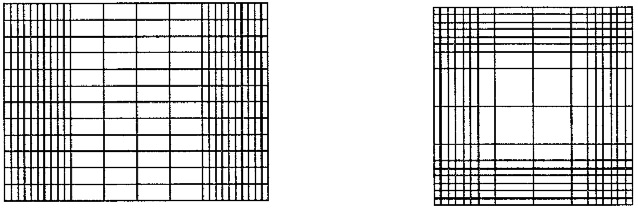
\includegraphics{src/images/f06b}}
    \caption[Bifocal Displays]{Bifocal Displays: distortion by linear function. From  \cite{Stroe1999}.}
    \label{fig:bifocal}
\end{figure}
\textit{Fish-eye Views} (figure \ref{fig:fisheye}) (also known as Table and Magnification Lense) apply a power function.
\begin{figure}[H]
    \centering
        \scalebox{.25}{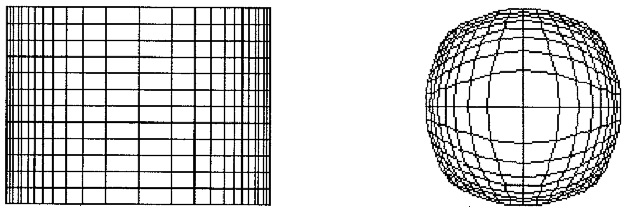
\includegraphics{src/images/f11c}}
    \caption[Fish-eye]{Fish-eye views:  distortion by a power function with an odd exponent  \cite{Stroe1999}.}
    \label{fig:fisheye}
\end{figure}

\textit{Perspective walls} (figure \ref{fig:perspectivewall}) distort the space by applying both linear and power function. Thus, a 3D-representation consisting of three walls is created. The front wall shows details and the two side walls provide context. 
\begin{figure}[H]
    \centering
        \scalebox{.25}{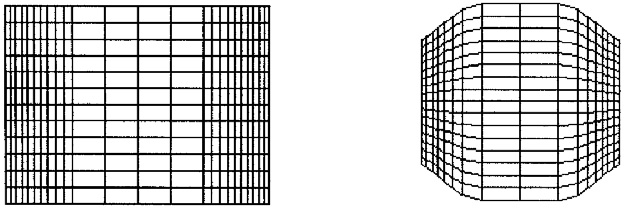
\includegraphics{src/images/f10b}}
    \caption[Perspective Walls]{Perspective Walls: distortion by a half linear and half power function. From  \cite{Stroe1999}.}
    \label{fig:perspectivewall}
\end{figure} 
\par
\textbf{Navigation techniques }include Brushing \& Linking \cite{Tegarden1999, Aigner2011}, Navigational Maps \cite{Keim2005} and Search \cite{Buono2005}. \\
\textit{Brushing \& Linking: }The user can select data items on the screen (Brushing) and the respective items are highlighted in every connected window (Linking) which is also known as coordinated window. Therefore, lasso, rubber-band or rectangular selection enables the user to select groups of data items. 
\par
Time-related interaction techniques are covered in \cite{Buono2005}. Buono et al. describe the system \textit{TimeSearcher} and the implemented interaction techniques for time-oriented data such as time-boxes. One interaction technique is pattern search. The user can draw a rectangular search box. The defined pattern is then searched in the data. Pattern search is one implementation of search as a navigation technique.\\
\par
In summary, all methods for clutter reduction in visualization tools support the business user in reducing information complexity. The proposed techniques can be divided into data reduction, visualization and interaction methods which is why this thesis applies this structure.
\par
\subsection{Big Data \& visualization tools}
% Topic: Survey of visualization tools
In chapter \ref{chap:Tools} we are comparing different \textbf{visualization tools}  and their ability to display large data. Wang et al. conclude that Big Data visualization tools perform poorly\cite{Wang2015}. In recently years many tools have been developed that promote themselves as able to handle Big Data \cite{Zoomdata2017, Datameer2017, Zeppelin2017}. Bikakis et al. surveyed different generic visualization systems and graph-based systems in the semantic web of Big Data \cite{Bikakis2016}. They compared the spectrum of analytical methods and visualization techniques. However, these systems are usually not used in business. 
Other tool comparisons are published by Zhang et al.  \cite{Zhang2012} and Patil  \cite{Patil}. These works compared commercial visual analytics system in the era of Big Data. Their key finding regarding visualization was the lack of support for advanced visualizations \gls{ADV}. In contrast Harger et al. surveyed open source visual analytics systems  \cite{Harger2012}. For \gls{BI} and Analytics the technology research center Gartner annually publishes a market overview of the most important \gls{BI} and Analytics tools which also serve for data discovery. The leading tools also appear in the survey  \cite{Evelson2012} regarding commercial advanced visualization tools and the works of Zhang  \cite{Zhang2012}. 
\par
In our work we survey time-oriented visualization techniques with regard to their scalability, makig use of existing taxonomies and scalability techniques. Our selection of tools were partially analyzed in other publications. However, the set of assessed criteria differed from ours.








\chapter{Related Work}
\label{chap:related Work}
In this chapter we provide an overview about the current literature which intersects with the topic of our work, the visualization of large time-oriented business data. Therefore, we consider the four influencing factors: business, time-oriented data, large size and surveys of visualization tools. 

% Business Information Visualization: Tegarden, Bačić
\subsubsection*{Business Information Visualization} 
Business Information Visualization (BIV) is defined as the use of visualization technologies to visualize business data\cite{Tegarden1999}. Although Information Visualization is intensively researched\cite{Shneiderman2008,Shneiderman2002,Shneiderman1996,Keim2002} only few researchers published to Business Information Visualization itself. While Tegarden\cite{Tegarden1999} introduced the most common definition of BIV and covered appropriate visualization techniques Bačić explored the process of knowledge creation\cite{Bacic2012} and how Business Intelligence can support business decision-making\cite{Bacic,Bacic2012}. Zhang\cite{Zhang,Zhang1998,Zhang2001} published a generalized visualization model in which she described the scope: BIV on the one side has to deal with non-geometric data and on the other side consider the human problem-solving process. This human centered perspective covered by Ware\cite{Ware2012a} as he examined how to design information visualization for human perception.

\subsubsection*{Large Scale Information Visualization}
The topic of information visualization for large data is studied by a broad number of researchers. While some works tackled the problem of reducing data others invented visualization techniques to display as much data as possible without aggregation\cite{Krzywinski2009,Luo2012,Fekete2002}. Important work was published by Keim\cite{Keim1996}. He proposed five categories for visualization techniques: pixel-oriented\cite{Keim1995,Stein2013,Keim2000,keim1996pixel,Keim2001, Keim2005,Keim2008VisualChallenges}, icon-based\cite{Chung2014,Borgo2013,Fanea2005}, hierarchical\cite{Yang2003,Shneiderman1992,LeBlanc1990}, graphic-based and geometric\cite{Noirhomme-Fraiture2002}.
A way to measure the scalability of large databases was defined with the term visual scalability. Visual or perceptual scalability is defined as the capability of visualization tools in displaying large datasets in an effective manner\cite{Eick2002}.
Interactions with large databases are covered in \cite{Fisher2012,Buono,Jerding1998,mackinlay1991perspective,Keim2005}. 

\subsubsection*{Time-oriented Visualization}
Data which is linked to time appears in the literature with various names: time-dependent\cite{Postfach2003, Tominski2005,Kriglstein2014,Aigner2007,VanBuuren2001,FerreiradeOliveira2003,Yang2003,Chung2014,Rind2011}, time-varying\cite{Moere2004}, time-oriented\cite{Aigner2008,Aigner2007,Aigner2011,Hinum2005,Walker} or time-related\cite{Keimc}. Significant work to the visualization of time-oriented data was done by Aigner\cite{Aigner2011,Aigner2008,Aigner2007}. They proposed a taxonomy for the time-domain and various visualization techniques. Other differentiations concerning time was made by \cite{Kriglstein2014}. They collected experimental findings for animation and space-metaphors for time. These studies compared animation, small multiples and traces. Yet, they found that none of them is able to scale beyond 200 data items\cite{Robertson2013}. Instead they suggested to use abstraction for analyzing large time-oriented datasets. Moreover, there exists a lot of ongoing research for univariate time-oriented data called time series\cite{Aigner2011, Buono, Walker,Leonard,Chen1993,Esling2012}.

\subsubsection*{Visualization Tools}
In the last chapter we will compare different visualization tools and their ability to display large data. In a survey to the Semantic Web generic visualization systems and graph-based systems have been surveyed\cite{Bikakis2016}. They compared the spectrum of analytical methods and visualization techniques. Yet, these systems are usually not used in business. Every year Gartner publishes a market overview of the most important Business Intelligence(BI) and Analytics tools which also serve for data discovery. The leading tools also appear in the survey\cite{Evelson2012} regarding commercial advanced visualization tools and the works of Zhang et al.\cite{Zhanga} and Patil\cite{Patil}. These work compared commercial visual analytics system in the era of Big Data. In contrast Harger et al. surveyed open source visual analytics systems\cite{Harger}. All the surveys consider visualization, interaction and analysis capabilites.

\subsubsection*{}
This work will contribute to the visualization of large data by focusing on time-oriented data. We will study different visualization techniques for time-oriented data in business and point out requirements for visualizing large time-oriented data in visualization systems. In a next step, visualization tools which are used in business, are selected and the requirements are checked. Finally, we give a recommendation for the tool use depending on the ease-of-use and programming skills and show further research topics.

\chapter{The challenge of large time-oriented data in Business Information Visualization}
\label{chap:BIV}


\iffalse
\listoftodos

\section{Outline} \todo{Remove from BA}
\begin{enumerate}
    \item The role of InfoVis in Business. Visual Analytics. Selfservice. Insights in Company/ Business. $\Rightarrow$ Business Data
    \subitem But: Other data types also in Business: IoT. Not covered because it is a too wide topic.
    \subitem Business use VA tools to get insight into data.
    \item Need for good visualizations for Business data
    \subitem What are business data? $\Rightarrow$ data types
    \item 2nd challenge: BigData.
    \subitem Where does BigData occur? Application Areas. Streaming Data
    \subitem Is BigData relevant for Business Data? Application Areas of Business Data
    \item Solutions in Literature
    \subitem Aggregation
    \subitem Abstraction
    \item Tools in Business
    \subitem Requirements: Visual Analytics Tools
    \subitem New Visualization Techniques -> Extensionability (p.12, "open
framework fed with pluggable visual and analytical components for analyzing
time-oriented data is useful. Such a framework will be able to support multiple
analysis tasks and data characteristics, which is a goal of Visual Analytics."
\cite{Aigner2007})
    \subitem Market Relevance: Qlik, Tableau
    \subitem Other Approaches: Jaspersoft(because its scalable),
    \subitem Comparison
    \item Conclusion: Which tool for time-oriented data?
\end{enumerate}
\fi

%%%%% Problems %%%%%%%%%%%%%
The visual data exploration of large time-oriented data in business evokes new requirements for visualizations. In this chapter we describe these requirements. Following a problem-oriented approach the first three sections outline the basics. Section \ref{problems} sketches the problems of visual clutter while section \ref{data} addresses the data and section \ref{tasks} the user tasks. In section \ref{vis} scalable time-oriented visualizations are explored and other factors influencing Big Data visualization are derived \ref{factors}. The visualizations and the factors together result in an advice for tools to visualize large data.
 \section{Understanding the problem}\label{problems}
 Nowadays, the challenge in BIV is to handle large amounts of data and displaying them in an effective manner. Yet, large amounts of data causes conflicts with effective data representation. One conflict is visual clutter. Visual clutter denotes overlapping and distracting data items. Clutter is caused by similar data items which overlap. If similar yet not identical data items are visualized at once items cannot be distinguished anymore. One example is shown in the figure below where clusters cannot be identified.
 
 \begin{figure}[H]
 \centering
 \begin{subfigure}[b]{0.25\textwidth}
     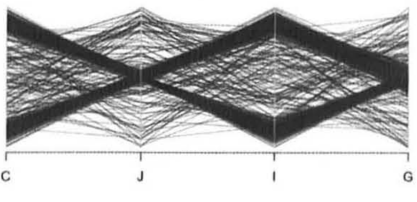
\includegraphics[width=0.20\textwidth]{src/images/PC1}
     \caption{Parallel Coordinates with clusters. From \cite{Tatu2010}.}
 \end{subfigure}
 \hfill
 \begin{subfigure}[b]{0.25\textwidth}
     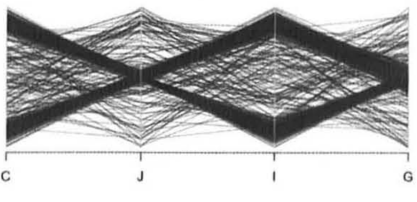
\includegraphics[width=0.20\textwidth]{src/images/PC1}
     \caption{Parallel Coordinates with clutter. From \cite{Tatu2010}.}
 \end{subfigure}
 \caption{Visual Clutter as a problem for data exploration}
 \label{fig:visual clutter}
 \end{figure}
 

 Visual clutter appears if the complete data set is displayed which is necessary to provide the user with overview. Shneiderman defined the importance of overview for visualization in its mantra: \textit{"Overview first, zoom in and filter, then details on demand} \cite{paterno1997concurtasktrees, Shneiderman2008, Keim2008}. Overview is a basic yet important task because it navigates the user in the data and allows further analysis. Thus, the problems of large data can be summarized as follows: 
\\*
\textit{Overlap}: 
The visualization of large data causes overlap. Depending on the drawing order the picture may look different and cause different interpretation even though the underlying data is the same. Visualization techniques need to avoid visual overlap (\ref{vis}, \ref{multi-resolution}). 
\\*
\textit{Visual Noise}: 
Even if data items are not overlapping data in large data sets might be to similar to each other. Thus, the user cannot differentiate distinct items on the screen. A solution is discussed in \ref{aggregationmarkers}.
\\*
\textit{Limited monitor resolution}:
Even if large monitors are used to visualize data in the end the available pixels on the monitor is smaller than the number of data items in a data set. This problem will be discussed in \ref{resolution}.
\\*
\textit{Limited visual perception}:
Moreover, human perception is limited in the numbers of patterns and pixels which will be reviewed in \ref{perception}.
\\*
\textit{Finding region of interest}:
If the data set is too large and overlap occurs the user faces the challenge of finding an interesting subset in the data. Thus, appropriate interaction techniques are necessary (\ref{search}).
\\*
\textit{Navigation}:
To find a region of interest the user might zoom in. But then another challenge occurs in navigating in the large data set. As there are too many data points the user might loose the overview and get lost in data analysis. Navigation techniques are a method to overcome this problem (\ref{navigation}).
\\*
\textit{Data Manipulation}:
If data is too large the user cannot identify whether the data is lying or not. Thus, the user may not detect data manipulation.
\\*
\textit{Information Loss}:
While reducing the number of data items to present them on the limited screen informations in the data can be lost. The important question is which data characteristics to keep such that the user tasks still can be supported.
\par
To propose a solution to the problems of large-scale data visualization it is important to gain understanding of the process of visualization which is described in the Visualization Pipeline. 
\begin{figure}[H]
    \centering
        \scalebox{.5}{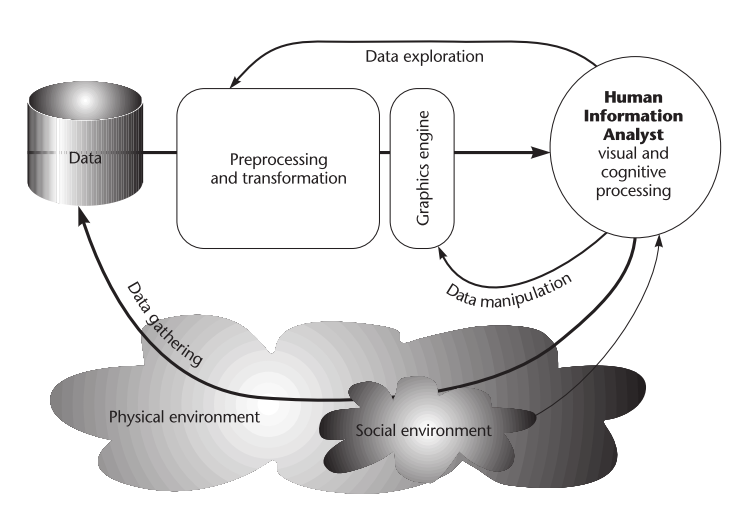
\includegraphics{src/images/VisPipeline}}
    \caption{Visualization Pipeline}
    \label{fig:vispipeline}
\end{figure}
Given the data as input visual clutter can be reduced by adapting the steps \textit{preprocessing \& transformation}, \textit{graphics engine}, \textit{visualization} and \textit{data manipulation}. Preprocessing involves data preparation as database joins or data cleansing. The graphics engine covers rendering processes and data formats. This part will not be covered in this work as it goes beyond the scope and the focus of this work is on visualization techniques. With visualization techniques are considered and data manipulation describes interaction techniques.  

Business visualization is used in the process of \textit{problem-solving}\cite{Bacic2012}. Thus, the user visualizes data to gain insights in the data and to find answers to formulated questions.  
As the visualization pipeline shows, the process of visual analysis is influenced by three entities: the data, the user and the visualization.
The three entities also can be described as \textit{domains}: data-domain, user-domain and visualization-domain. The data-domain represents \textit{what} is visualized. The user-domain explains \textit{why} the problem is visualized and the visualization-domain characterizes \textit{how} the problem is visualized. Thus, we will now explore the three domains to answer the following questions: 

\begin{itemize}
    \item What is presented?
    \item Why is it presented?
    \item How it is presented?
\end{itemize}


% Data types for Information Visualization
\section{Data type} \label{data}

\textbf{What is presented?}\\*
Talking of large time-oriented data for business we will consider the three given characteristics of the data: characteristics of business data, time-dependency and their size. Business data is collected in many different areas. The following table gives an overview about the applications: 

\begin{table}[H]
	\centering
	\caption[Business Applications]{Business Applications\cite{Brachman1996,Tegarden1999}}
	\label{businessapplications}
	\begin{tabular}{ll}
	\toprule
	Marketing & Financial Sector \\
	Fraud Detection & Manufacturing and Production \\
	Operations Planning & Market Analysis \\
	Health Care & Network Management\\
	\bottomrule
	\label{table:applications}
	\end{tabular}
\end{table}
For each application area exists a number of publications covering different aspects. Thus, the analysis of every single application would go beyond our scope and we decided to consider data with the following characteristics: 
\begin{enumerate}
    \item The data is structured. 
    \item The data is abstract.
    \item The data is multivariate.
    \item The data is discrete.
\end{enumerate}
These assumptions are based on the work of Tegarden in which business data is described as abstract and multivariate and discrete\cite{Tegarden1999}.
\textbf{Structured data}: Data can come in many different forms. Unstructured data appears in text, speech and language processing\cite{Borgo2013}. Structured data comes in tables in which each attribute are represented by one column and each row is one data item. The attributes can be either numerical or text-based. As multivariate data is usually presented in tables\cite{Borgo2013} we assume that business data is structured.\\*
\textbf{Abstract data}: Abstract data is defined as data without any spatial relationship in the data\cite{Shneiderman1996}. \\*
\textbf{multivariate data}: 
Often, multivariate is mixed-up with the term multi-dimensional. For this reason we define  multivariate data by the number of dependent attributes. If the data set holds more than two dependent attributes then we call the data \textit{multivariate}. In contrast, multi-dimensional depicts the number of independent attributes of a data set\cite{Aigner2011}.  \\*
\textbf{Discrete and time-oriented data}: A time-oriented data set contains data items which change over time. Each data item has a timestamp which is saved in one table-column. The time-dependency of the data structures the data by a given order. Every data item is mapped to a specific point in time with a smallest possible unit such as seconds. Time with a smallest unit is mapped to integer\cite{Aigner2011} and thus we assume that time-oriented business data is discrete and has a given order.  \\*

In section \ref{vis} different techniques are compared which were selected when they could display time-oriented abstract, multivariate and discrete data. 
Time-oriented data can characterized further into linear or cyclic, point- or interval-based and branching or muliple perspective\cite{Aigner2011}. These factors where not considered in the selection of techniques. \\*

\textbf{Large data:} To characterize the data volume we stick to a definition of Huber. He divided data in small, medium, large, huge and massive data. Large data according to\cite{Huber1994} is defined as data sets with $10^6$ and huge data with $10^8$ data entries. We are considering large and huge amounts of data. Nowadays, companies strive to do \textit{Big Data}. Big Data in typically defined as data with  high volume, high velocity, high veracity and high variety\cite{Wang2015}. The contribution of our work to Big Data is the study of visualization of high volume data sets.



% User Tasks
\section{Time-oriented User Tasks} \label{tasks}
\textbf{Why is it presented?}\\*
In the visualization analysis process the user has the role of the data analyst. Thus, every visualization tool should consider the user perspective. The business user is a kind of person which is interested in verify existing hypothesis (verification) and discover new patterns (discovery). By using the tool he expects the tool to assist him in analyzing the data, finding critical points and perform analysis automatically\cite{Brachman1996}. Verification and discovery in the analysis of time-oriented data can be split in seven major tasks\cite{Esling2012}:\\*

\textbf{T1: Query by Content}
\\*
Given a known query \textit{query by content} describes the retrieval of similar items to this query. In time-oriented data query by content returns the \textit{k} most similar time series to the queried time series.
\\*
\textbf{T2: Clustering}\\*
Clustering is the process of finding expressive groups (clusters) out of the data. Therefore, the data set is divided into subgroups according to some similarity measure. In the context of large time-oriented data clustering is important to compare similar time-series.
\\*
\textbf{T3: Classification}\\*
In classification the task is to find the right group the item belongs to. According to \textit{Aigner et al.} temporal classification describes the preprocess of finding the correct group for given data or data set. This task is important for large data to abstract the data and make them handable. As this task is preprocessing and not data presentation or exploration we will not check whether the tools support the user in this task. 
\\*
\textbf{T4: Segmentation}\\*
Segmentation splits a time series into \textit{k} meaningful subsequences (segments)\cite{batyrshin2007perception}. 
\\*
\textbf{T5: Prediction}\\*
In Prediction\textit{k} future events are predicted based on the past \textit{n} time series. This process is also known as \textit{forecasting}. 
\\*
\textbf{T6: Anomaly Detection} \\*
Anomaly detection points out events which behave in a different way than expected.
\\*
\textbf{T7: Pattern Discovery} \}\*
Pattern discovery finds regularly appearing structures in a time series.  It covers the exploration of trends, outliers and clusters. Especially, in business this task is one the most important tasks.


% Visualization Techniques
\section{Visualization of large-scale time-oriented Data} \label{vis}
\textbf{How is it presented?}\\*
% introduction of methodology: selection of vizTechniques, introduction of classes
The following section discusses several visualization techniques for time-oriented data with regard to their scalability to large data sets. The choice of the technique influences the scalability which is illustrated by the following example. 
A line chart maps one dimension to the x-axis while a second dimension is mapped to the y-axis as in figure \ref{fig:linechart}. Considering, that each data items requires one screen pixel the maximum number of data items is limited by the window width. 
\begin{figure}[H]
    \centering
    \scalebox{0.2}{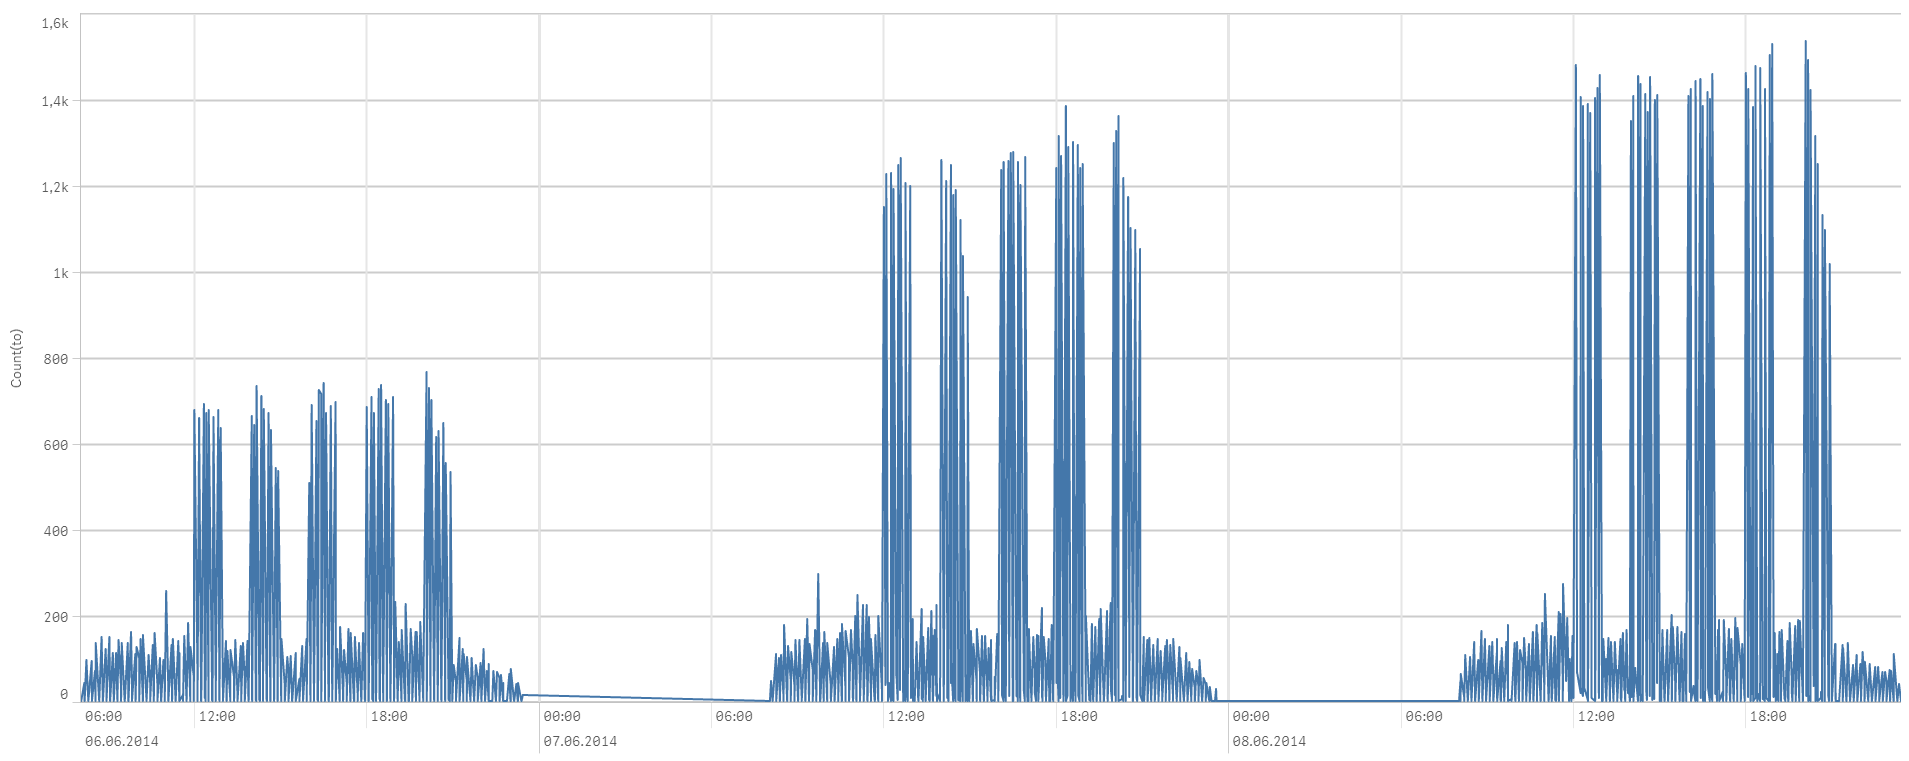
\includegraphics{src/images/linechart}}
    \caption{Linechart}
    \label{fig:linechart}
\end{figure}
 
In contrast to the line chart uses the scatter plot three attributes and thus, the maximum number of data items in the scatter plot exceeds the maximum in the line chart which is shown in \ref{fig:scatterplot}. Thus, the technique influences the maximum number of data items. 
\begin{figure}[H]
    \centering
    \scalebox{0.2}{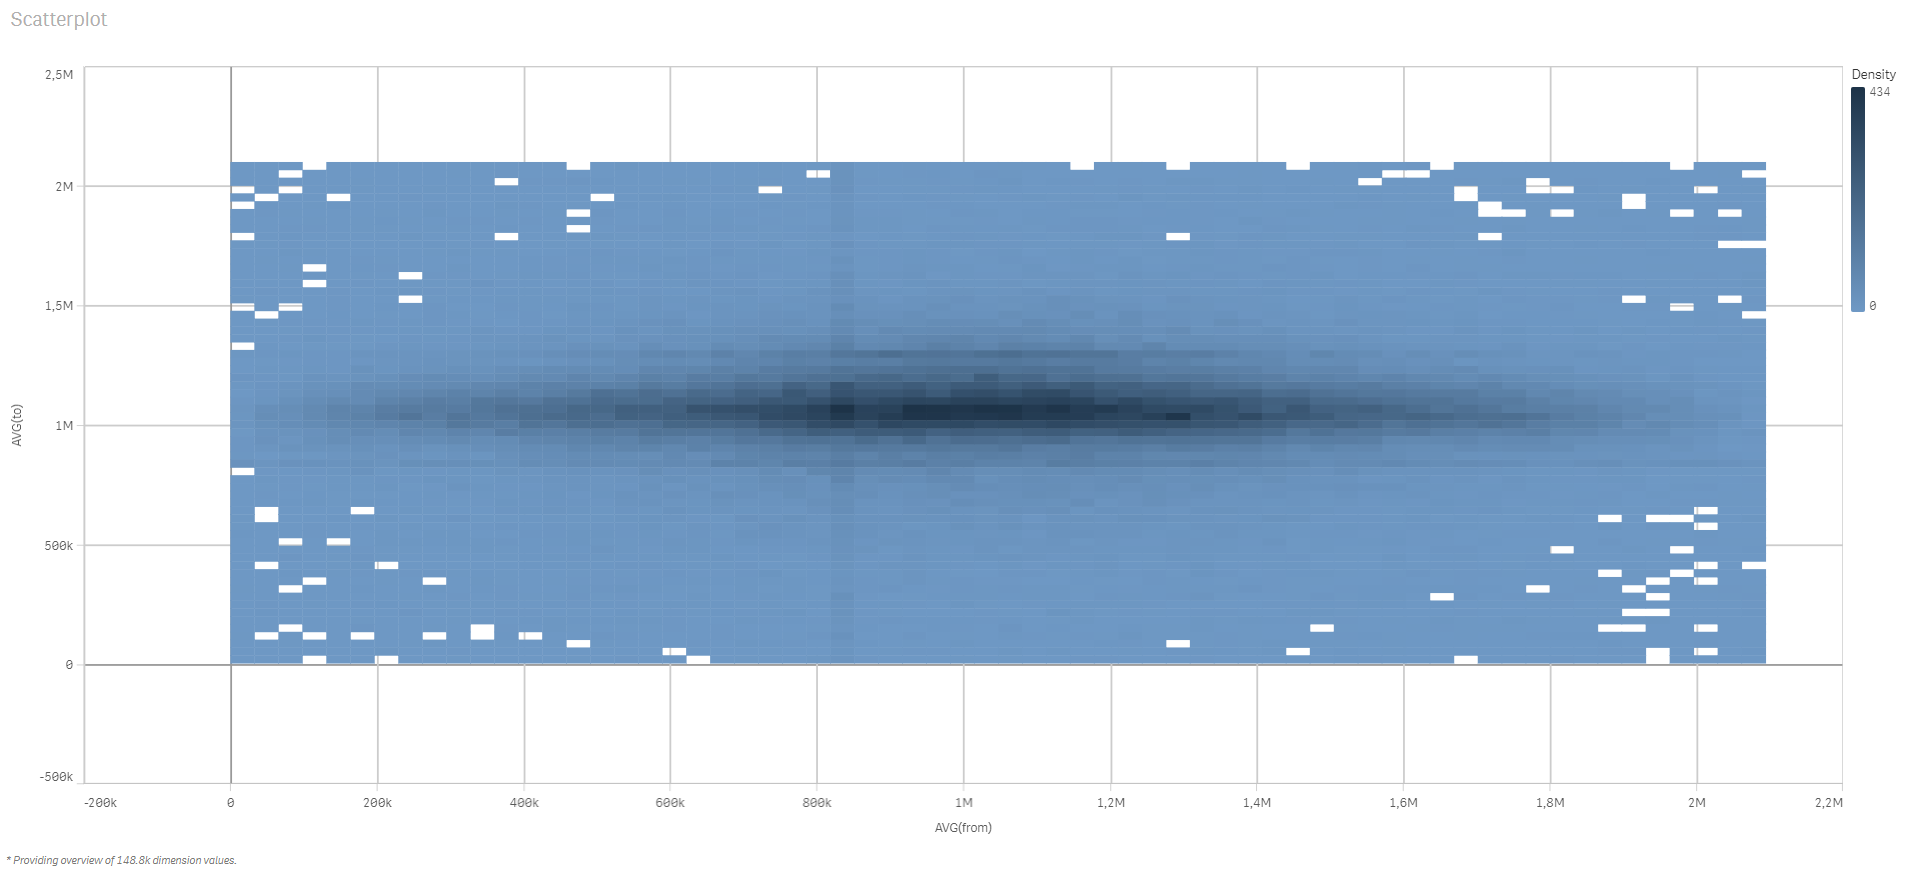
\includegraphics{src/images/SmartDataCompression}}
    \caption{Scatter plot}
    \label{fig:scatterplot}
\end{figure}
 

\textbf{Standard Visualizations of time series data}
Usually time series data is visualized with line charts. However, line charts can only show \textit{univariate} data. Our selection of visualization techniques is based on Aigner et al.\cite{Aigner2011} which presents current approaches to visualize time-oriented data. Hereby, we focus on 34 techniques which can be used to show abstract, multivariate and discrete data (compare section \ref{data}). 
As the work of Aigner was published in 2011 we completed the set of techniques with current approaches based on the \href{http://survey.timeviz.net/}{TimeVizBrowser}. Moreover, we consider only stand-alone visualization techniques which are techniques no systems, tools or software. In literature a significant amount of publications describe new tools or systems which tackle the visualization of time-oriented data. These tools usually are specific tools which can only be applied in a limited field. As we write this work with the perspective of business users tools have to be generic and single-task systems are not appropriate.

We are aware that this discussion cannot be exhaustive as time-oriented data is a current research area and day-to-day new visualization techniques are developed.
Moreover, time-oriented data appears in different areas of business: E-commerce, Smart Health, E-Government, Science \& Technology, Security \& Public safety. Each sector collects different types of data and uses different applications, which makes it impossible to name every single existing visualization technique.


However, we think that this work gives a good overview of visualization techniques as we stick to Keim's taxonomy\cite{Keim1995} of visualization techniques for large data which classifies visualizations into the following classes: \textit{geometric-projective}, \textit{graph-based}, \textit{hierarchical}, \textit{icon-based} and \textit{pixel-oriented}.
\\*
\textbf{Graph-based} techniques present large graphs by using layout algorithms\cite{Keim1996}.\\*
\textbf{Geometric projection} techniques (GP-techniques) map multi-dimensional data to the 2D screen\cite{FerreiradeOliveira2003}.\\*
\textbf{Pixel-oriented} techniques map each data item to one pixel on the screen. Position and color are used to represent data attributes\cite{Keim1996}.\\*
\textbf{Hierarchical} techniques divide the k-dimensional space into subspaces and shows them hierarchically. \\*
\textbf{Icon-based} techniques map each data item onto one icon. The attributes are mapped to different icon features\cite{Keim2001}.



\subsection{Visual Scalability}\label{scalability}

This work studies how well these techniques scale to large data. To define the ability of visualizations to present large amounts of data we introduce the term \textit{visual scalability}.
Visual or perceptual scalability is defined as the capability of visualization tools in displaying large data sets in an effective manner\cite{Eick2002}\label{effective}. In the context of time-oriented business data effective means the presentation of patterns to support the user tasks. To measure the visual scalability of different visualization techniques for time-oriented data we refer to the work of Eick\cite{Eick2002}. He proposed to measure visual scalability by the database metrics of the data set and the visual characteristics of the visualization technique. \\*
\textbf{Database metrics}\label{databasemetrics} measures the \textit{size of the database} in bytes, the number of rows or the number of attributes at the level of the visualization tool. For multi-dimensional data the \textit{database metrics} are a combination of the number of rows and the attributes. \\*
\textbf{Visualization characteristics} describe the number of elements and attributes presented on the screen, thus measuring how many distinct items a visualization technique can display. This number is measured on the visualization technique level.\\*
The combination of the database metrics and the visualization characteristics describes the scalability of a visualization tool. Furthermore, the tools scalability is influenced by more factors which will be discussed later (\ref{factors}).

\subsubsection{Visual Scalability of time-oriented techniques}\label{visualization}
The analysis of visualization techniques showed that time-oriented techniques are classified in only four of Keim's visualization classes: geometric, hierarchical, icon-based and pixel-oriented. In the following table we will name the corresponding techniques for multivariate time-oriented data. Subsequently, we will discuss the visualization characteristics for each class. 


\begin{table}[H]
	\centering
	\caption[Visualization Classes]{Visualization Classes}
	\label{vizScalability}
	\begin{tabu}{  | l | l | l |}
	\toprule
	Visualization Class & Technique & References\\
	\midrule
	    \multirow{8}*{Geometric} 
		& EventRiver        & \cite{Luo2012}\\
		& Flocking Boids    & \cite{Moere2004}\\
	    & Kiviat Tube       & \cite{Tominski2005}\\
        & MultiComb         & \cite{Tominski}\\
        & Multi-resolution CircleView & \cite{Keim2005}\\
        & Parallel Glyphs   & \cite{Fanea2005}\\
        & Temporal Star     & \cite{Noirhomme-Fraiture2002}\\
        & TimeWheel         & \cite{Tominski}\\ \hline
        \multicolumn{3}{|p{\linewidth}|}{
        The visualization characteristics of geometric projection techniques (GP-techniques) strongly depend on the mapping-function which regulates the projection of multi-dimensional data to the 2D screen\cite{FerreiradeOliveira2003}. The mapping-function often includes data reduction techniques (see section \ref{analytical}).  When data reduction techniques are involved, this class of techniques is able to visualize large to huge data sets. This class will be described in detail (\ref{GP-Techniques}).} \\ \hline
        
		\multirow{3}*{Hierarchical} 
		& Pixel-Oriented Network Visualization  & \cite{Stein2013}\\
		& Software Evolution Analysis   & \cite{Gall}\\
		& Timeline Trees                & \cite{Burch}\\ \hline
		\multicolumn{3}{|p{\linewidth}|}{We analyzed three hierarchical visualization techniques. Timeline Trees included aggregation techniques by collapsing nodes. With collapsed nodes the technique can display large to huge amounts of data. Pixel-oriented Networks use clustering and thus, \todo{Begrüdung für Skalierbarkeit einfügen}} \\ \hline
        \multirow{5}*{Icon-based}
        & Gravi++       &\cite{Hinum2005}\\
        & InfoBUG       &\cite{chuah1998information}\\
        & PeopleGarden  &\cite{xiong1999peoplegarden}\\
        & Spiral Graph  &\cite{Weber2001}\\
        & VIE-VISU      &\cite{horn2001support}\\ \hline
        \multicolumn{3}{|p{\linewidth}|}{
        As every data item requires one icon icon-based techniques can show less data items than the number of pixels on the screen. When showing large data icon-based techniques face the challenge of clutter and occlusion\cite{Borgo2013}. Thus, icon-based techniques can only display small- to medium-sized data sets.}\\ \hline
        \multirow{12}*{Pixel-oriented}
        & 3D ThemeRiver & \cite{Imrich2002}\\
        & Braided Graph & \cite{Javed2010}\\
        & CircleView    & \cite{Keim2005}\\
        & Data Tube Technique & \cite{ankerst2001visual}\\
        & history flow  & \cite{viegas2004studying}\\
        & Kaleidomaps   & \cite{bale2007kaleidomaps}\\
        & Pixel-Oriented Network Visualization  & \cite{Stein2013}\\
        & Recursive Pattern & \cite{Keim1995}\\
        & Spiral Display    & \cite{Carlis}\\
        & Stacked Graphs    & \cite{byron2008stacked}\\
        & ThemeRiver        & \cite{Havre2000}\\
        & Time Curves       & \cite{Bach2016}\\
        & TimeRider         & \cite{Rind2011}\\ \hline
        \multicolumn{3}{|p{\linewidth}|}{
        Since only one pixel per data item is used this class can maximize the used screen space. Let $M$ be the monitor resolution with the screen-width $w$ and the screen-height $h$, $P$ the number of pixels in $M$ and $D$ the maximum of data which can be displayed at once. In pixel-oriented techniques  \begin{math}
        D = w*h
        \end{math}
        which shows that pixel-oriented techniques can display large, but not huge data.}
        \\ \hline
	\bottomrule
	\end{tabu}
\end{table}


Most of the existing visualization techniques nowadays still are not appropriate in visualizing huge data. Pixel-based visualizations represent each data item by one pixel and thus, are limited to 2 mio. pixels. Even new visualization techniques which where developed to visualize "very large" data sets follow the pixel-oriented approach\cite{Keim1995, Keim1996}. Icon-based visualizations display one data item per icon and thus can display even less data than pixel-oriented visualizaton techniques. The most promising techniques are hierarchical and geometric-projective techniques as they combine aggregation or abstraction with visualization. Their scalability depends on the mapping-function. 
One interesting extension of pixel-oriented techniques is the \textit{multi-resolution} approach\cite{Keim2005}. The idea is to show more relevant data items at a pixel-based level and less relevant data items in an aggregated way. The technique \textit{multi-resolution CircleView} shows recent data at full resolution in the middle of the circle and places previous-year-data  at the outer circle. With multi-resolution it is possible to extent the pixel-limit from $w*h$ to larger data sets. 

\begin{table}[H]
	\centering
	\caption[Scalability of Visualization Classes]{Scalability of Visualization Classes}
	\label{vizScalability}
	\begin{tabu}{ l | c }
	\toprule
	Visualization Class & Scalability\\
	\midrule
	Geometric &  \cellcolor{green!25 } > 2 mio. pixel\\
	Hierarchical & \cellcolor{green!25} > 2 mio. pixel \\
	Icon-based & \cellcolor{red!25} $\leq$ 1 mio. pixel \\
	Pixel-oriented & \cellcolor{yellow!25} $\leq$ 2 mio. pixel \\	
	\bottomrule
	\end{tabu}
\end{table}





%Aspects of Scalability:
% Wie viele Datenpunkte sind notwendig, um Pattern darzustellen? -> data 
% Interaction Techniques
% Downsampling -> Analytical Methods
\iffalse
 The challenges of large-scale data for ADV are \textit{scalability} and \textit{dynamics}\cite{Wang2015}. With its volume the challenges for large-scale data are also challenges for Big Data defined as high volume, high velocity, high veracity and high variety data sets\cite{Wang2015}. In this work we concentrate on the scalability challenge for visualization techniques. The challenge is in finding appropriate techniques\cite{Aigner2008,Keim2005} which scale to large amount of data.
 
\fi

\subsubsection{Visualization characteristics of GP-Techniques} \label{GP-Techniques}
Geometric-projective visualizations seems to be the most scalable visualization technique depending on the mapping function. For this reason we will explore techniques in the geometric-projective class in detail and discuss their scalability.


Furthermore, we suggest to divide GP-techniques into \textit{radial} and \textit{non-radial} visualizations\cite{Diehl2010} as our  analysis has shown that a large part of GP-techniques is based on a radial layout. Radial GP-techniques share common properties such as the maximum number of attributes which is set to 10-20 attributes\cite{Diehl2010}.\\*


\begin{table}[H]
	\centering
	\caption[Radial and non-radial GP-techniques]{Radial and non-radial GP-techniques}
	\label{radialTable}
	\begin{tabu}{lcc}
	\toprule
	GP-Technique & radial & non-radial \\
	\midrule
	Flocking Boids &  & x \\
	Kiviat Tube & x &  \\
	MultiComb & x &  \\
	Multi-resolution CircleView & x &  \\
	Parallel Glyphs & x &  \\
    Temporal Star & x &  \\
	TimeWheel & x & \\
	\bottomrule
	\end{tabu}
\end{table}

As discussed in \ref{scalability} the scalability of visualizations is measured by the number of distinct items. Distinct items are calculated with the maximum number of data items * the maximum number of attributes. 

\textbf{Flocking Boids} simulate the evolution of data items in 3D. Thus, data objects are represented by a colored, curved line with changing transparency called \textit{boid}.  A data object is an aggregation of same data items, e.g. one boid is one stock market company. A boid calculates the average of multiple data attributes and uses behavior rules to simulate the development of a data object. The rules define the position of data item over time and its velocity. Thereby, time is represented by animation and boids correspond to distinct items on the screen. Thus, the maximum measured number of used boids defines the scalability. Flocking Boids were able to handle 500 boids at a time. Thus the scalability of Flocking Boids is 500 which is low compared to pixel-oriented techniques(2mio items)\cite{Moere2004}.
Analytical Methods such as clustering or subset selection are outsourced to database algorithms and interaction techniques are not implemented but could be extended\cite{Moere2004}. 
\begin{figure}[H]
    \centering
        \scalebox{.3}{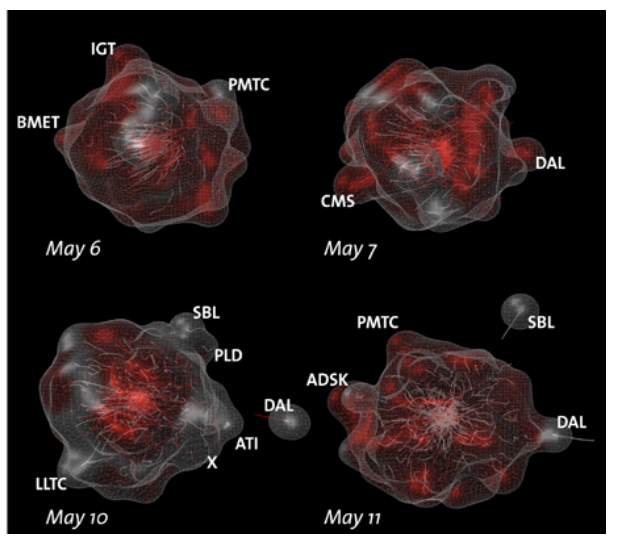
\includegraphics{src/images/FlockingBoids}}
    \caption{Flocking Boids. From \cite{Aigner2011}.}
    \label{fig:flockingboids}
\end{figure}
\\*
\textbf{Kiviat Tube} is an unfolded Radar Chart along the z axis in 3D. Several Radar Charts are stacked behind each other along the time (z) axis and form a tube. Thus, variables are mapped on radial aligned planes and can be compared. Interaction such as changing the planes positions and navigating through time enables the user to compare different variables over time.\\*
The number of attributes is limited to approximately 10-20 attributes as the radial layout limits the number of variables. As the Kiviat Tube is a 3D representation the tube is projected to the 2D screen. Let $w$ be the window width. Then, the maximum number of data items is $\leq w$ as the technique does not include any aggregation. The scalability is $20*w\approx 20.000$.
\begin{figure}[H]
    \centering
        \scalebox{.3}{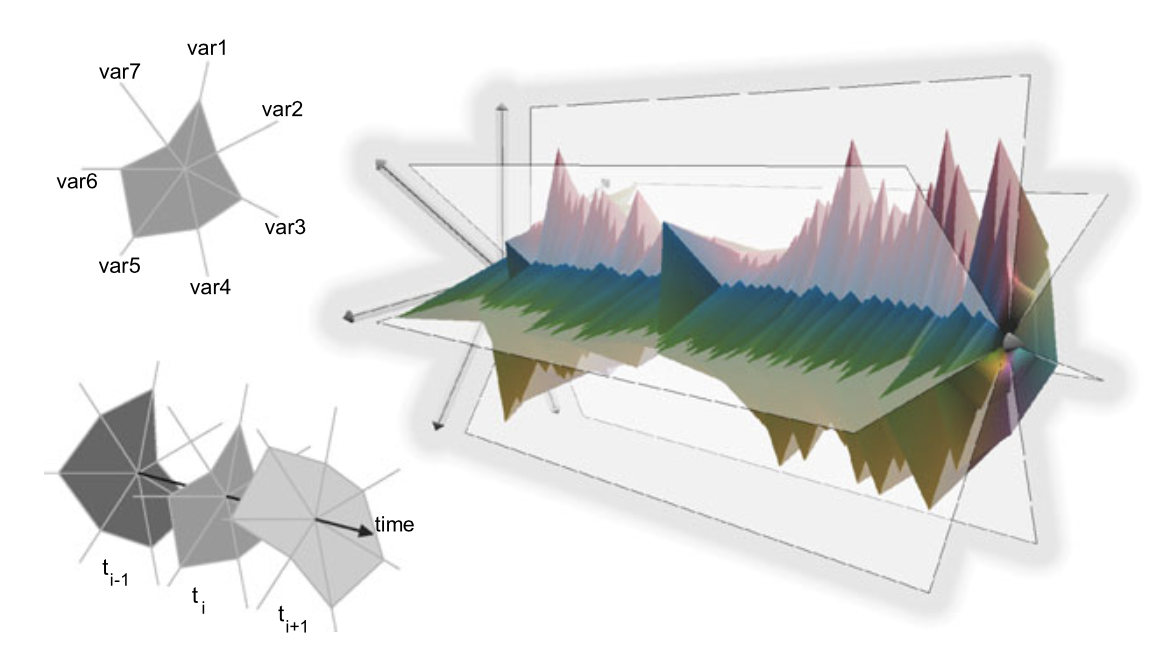
\includegraphics{src/images/KiviatTube}}
    \caption{Kivit Tube. From \cite{Aigner2011}.}
    \label{fig:kiviattube}
\end{figure}
\\*
In \textbf{MultiComb} \textit{k} time series plots are mapped on a circle in two possible ways. One way is to position the plots along the circumference. Or the plots are mapped perpendicular to the circumference. In this version the plot resembles a star.  The MultiComb is radial. Let $h$ be the window height, then the maximum number of data items in version two is $< \frac{h}{2}$ and the scalability $20*< \frac{h}{2} \approx 10.000$
\begin{figure}[H]
    \centering
        \scalebox{.3}{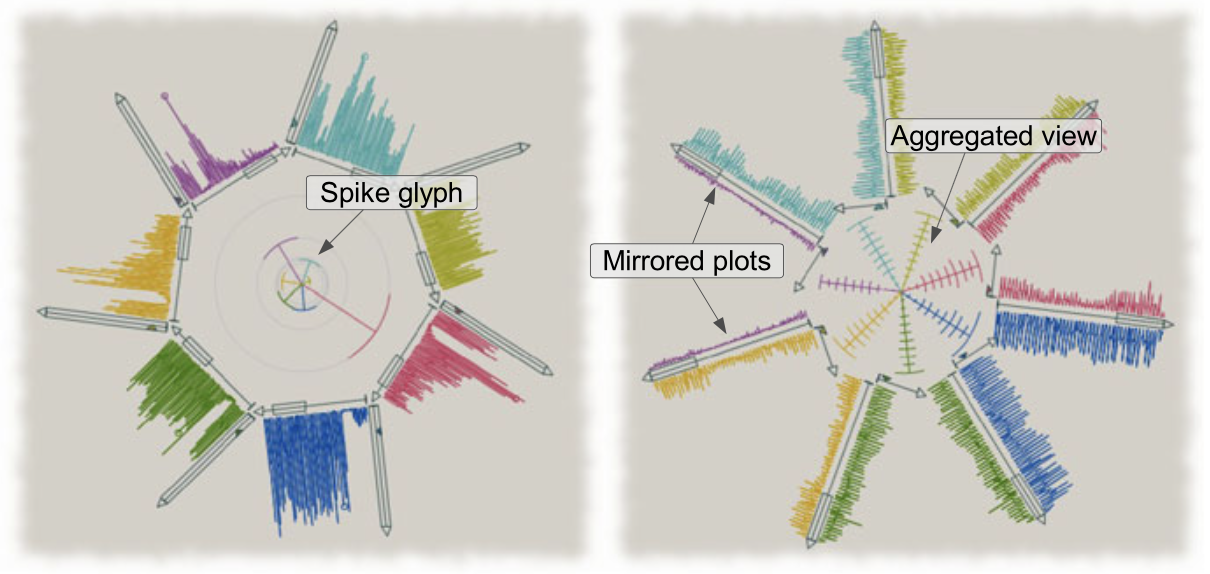
\includegraphics{src/images/MultiComb1,2}}
    \caption{Multi Comb. From \cite{Luo2012}.}
    \label{fig:multicomb}
\end{figure}
\\*
\textbf{Multi-resolution CircleView} enhances the CircleView technique. Instead of mapping each value to one pixel, data items are aggregated. More recent items are placed in the middle of the circle. These items are represented by one pixel each. Less relevant items are aggregated and placed at the outer part of the circle. These items are usually from a preceding point of time. As Multi-resolution CircleView uses aggregation the maximum number of data items is $> 2mio.$ pixels which makes multi-resolution circle view to a scalable visualization.
\begin{figure}[H]
    \centering
        \scalebox{.3}{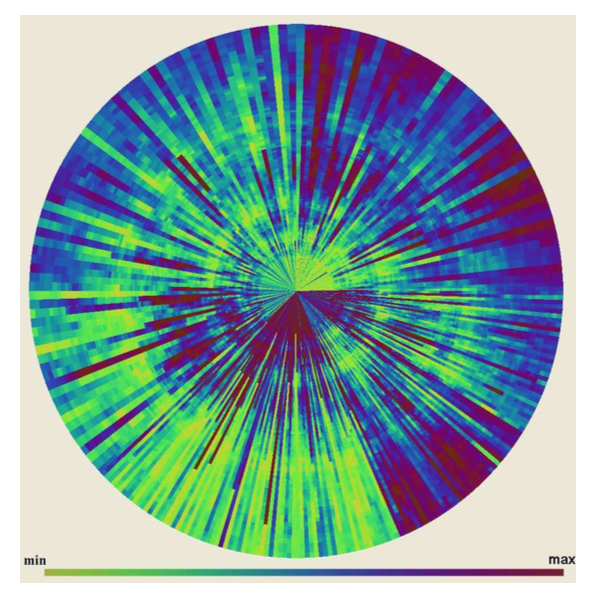
\includegraphics{src/images/MultiResolutionCircleView}}
    \caption{Multi-resolution CircleView. From \cite{Keim2005}.}
    \label{fig:multiresolutioncircleview}
\end{figure}
\\*
\textbf{Parallel Glyphs} pair Parallel Coordinates with Star Glyphs. While similar to Parallel Coordinates each data item is represented by a polyline which connects the vertical axis (attributes) the attribute axis are radially unfolded in 3D and show the data value of the data item over time. Thus, each data value over time is represented by a star glyph. The visualization can be expanded by connection lines over star glyphs. Parallel Glyphs provide brushing of polylines, filtering, axis reordering, rotating in 3 directions, transparency support if the glyphs overlap each other, focus+context presentation through magnification lenses. Through the extension of 2D to 3D parallel glyphs are able to display more data rows than parallel coordinates (PC). PC had the problem of clutter while displaying 15.000 data items on a gray-scale \cite{Keimb}. Yet, as the maximum number of data items is below one mio. data points parallel glyphs are no scalable visualization technique. 

\begin{figure}[H]
    \centering
        \scalebox{.3}{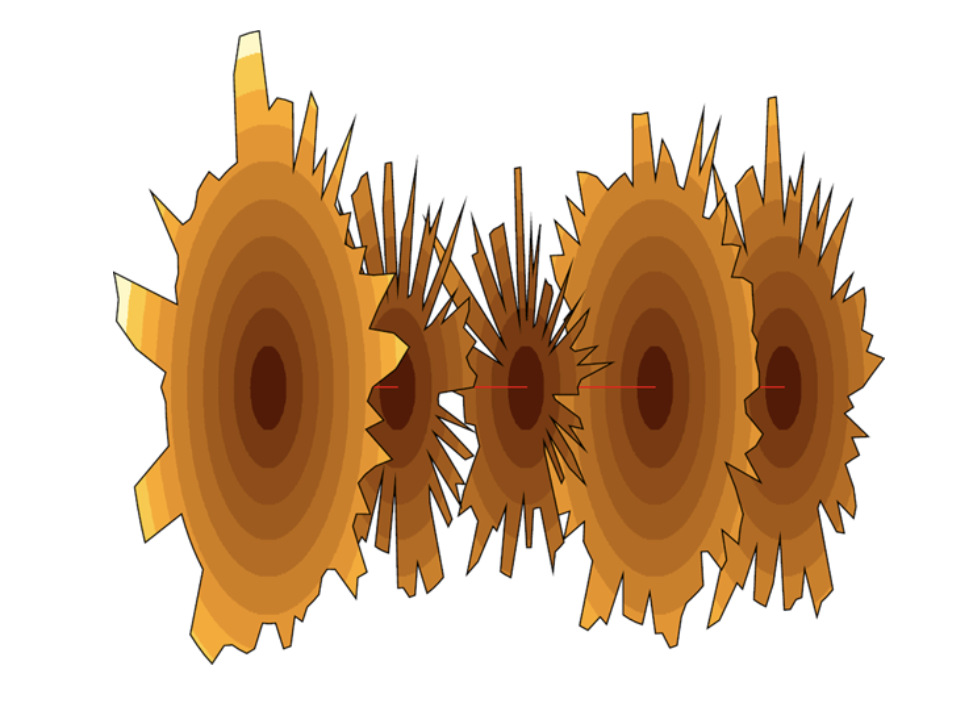
\includegraphics{src/images/ParallelGlyphs}}
    \caption{Parallel Glyphs. From \cite{Aigner2011}.}
    \label{fig:parallelglyphs}
\end{figure}\\*

\textbf{Temporal Star} aligns multiple attributes in a star-like manner around the centre. Each star is one point of time. The time axis connects several stars to a 3D-object. Temporal star uses so called \textit{symbolic objects} to display aggregated data. This way temporal star is designed to show large data sets. 
\begin{figure}[H]
    \centering
        \scalebox{.3}{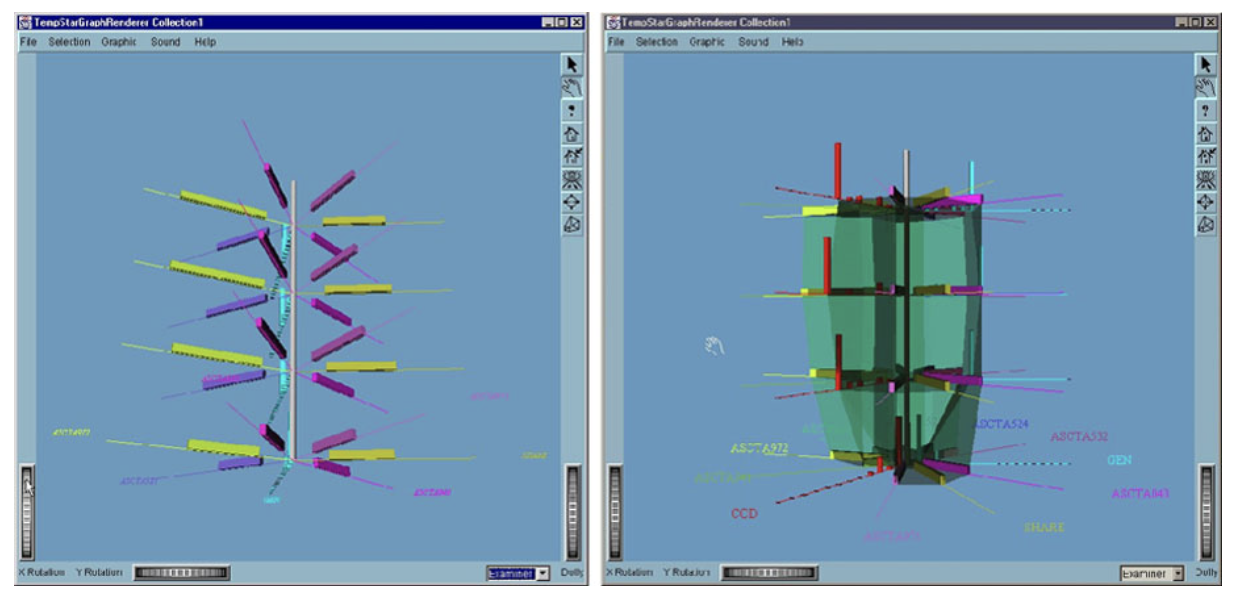
\includegraphics{src/images/TemporalStar}}
    \caption{Temporal Star. From \cite{Aigner2011}.}
    \label{fig:temporalstar}
\end{figure}\\*

\textbf{TimeWheel} is a 2D technique. Similar to variation one of \textit{MultiComb} attribute axis are positioned along the circle circumference. In the centre of the circle the time axis is placed. Let $a$ be the pixel width of this axis and $a < w$. Similar to MultiComb Time Wheel does not include aggregation and thus the maximum number of data items is limited to $a$. Thus, the scalability is $20* <w \approx 10.000$.
\begin{figure}[H]
    \centering
        \scalebox{.3}{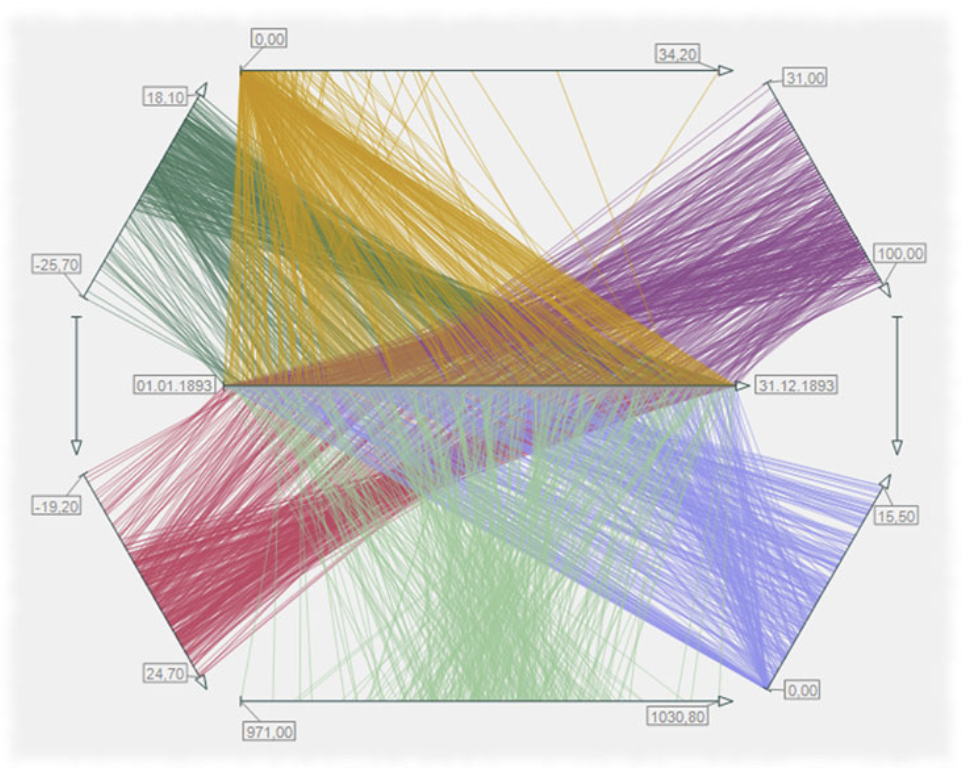
\includegraphics{src/images/TimeWheel}}
    \caption{Time Wheel. From \cite{Aigner2011}.}
    \label{fig:timewheel}
\end{figure}\\*

\begin{table}[H]
	\centering
	\caption[Scalability of GP-Techniques]{Scalability of GP-Techniques}
	\label{GPscalability}
	\begin{tabu}{lcc}
	\toprule
	GP-Technique & scalability \\
	\midrule
	Flocking Boids & \cellcolor{red!25 }500* \\
	Kiviat Tube & \cellcolor{red!25 }20.000 \\
	MultiComb & \cellcolor{red!25 }10.000 \\
	Multi-resolution CircleView & \cellcolor{green!25 }$>$ 2mio.\\
	Parallel Glyphs &  \cellcolor{yellow!25 }15.000 - $>$ 1mio.\\
    Temporal Star &  \cellcolor{green!25 }$>$ 2mio.\\
	TimeWheel & \cellcolor{red!25 }10.000\\
	\bottomrule
	\end{tabu}
\end{table}

Geometric-projective techniques are limited in the maximum numbers of items. Out of the four visualization classes \textit{multi-resolution CircleView, Temporal Star and hierarchical techniques} are appropriate to visualize large amounts of data. 
% TCS: Optimum for ADV 
In summary, visualization tools should integrate advanced data visualization (ADV) to visualize time-oriented multivariate data. In our understanding ADV is a visualization technique which is able to scale to large and huge amounts of data. \\*
%\textit{Aigner et. al} classify Parallel Coordinates as standard visualizations\cite{Aigner2011} whereas \textit{Keim et. al.} \cite{Keim} are talking about Parallel Coordinates as a novel technique. This discussion of course is determined by the time epoche. The longer a visualization technique is known the more it is counted as a standard visualization technique. 

However, only few techniques are able to represent billions of data. In the end, most of them are limited through the 2D-screen. Factors which enhance the scalability are \textit{advanced visual metaphors}, \textit{interaction techniques} and \textit{data reduction}. 



\section{More factors} \label{factors}
Moreover, besides the database metrics and the visualization characteristics visual scalability is influenced by six factors\cite{Eick2002}: 
\begin{itemize}
    \item Monitor Resolution 
    \item Human Perception\cite{Keim2005,Deering1998}
    \item Visual Metaphors
    \item Interactivity
    \item Data Reduction
\end{itemize}

\subsection{Monitor Resolution}\label{resolution}
Even though large wall-sized screens have been developed nowadays monitors with a display width of 50 cm are used in business. Sometimes, -depending on the department- two or three monitors are combined for a larger wall. Thus, the maximum number of pixels which can be used at the workspace ranges from 786.432 (1024x768) to 6.912.000 (3 monitors à 1920x1200).
Concluding, the available amount of data in a data set exceeds the maximal number of screen pixels by far. But, besides the available monitor resolution another limiting factor is the perceivable number of pixels by the human perception.

\subsection{Human Perception} \label{perception}
% What can humans perceive? How many pixels? 
The brain is limited in perceiving pixels on the screen as well as patterns created by visualizations. Since space in brain is represented different from the screen the term computer monitor pixels requires a brain equivalent for screen pixels. We call them brain pixels. According to \cite{Ware2012a} brain pixels are nearly represented by ganglion cells. Ganglion cells are neurons which send information to the cortex. In the fovea one ganglion cell cares about one single cone. In the periphery one ganglion cell handles thousand rods and cones. Thus, the brain pixel resolution in the fovea is much higher than in the periphery. The brain aggregates pixels and adheres multi-resolution. 
To model how many data items are perceived by the human brain it is important to make the following distinction: 
\\*
\textit{TBP = total amount of brain pixels which is stimulated by the screen pixels}\\*
and unique stimulated brain pixels: \textit{USBP = TBP - redundant brain pixels}.\\*
USBP are the number of pixel who determines the human perception of data items. A measure of display efficiency (DE) is the ratio of USBP and screen pixels(SP): \textit{DE = USBP/ SP}.

\begin{figure}[H]
    \centering
    \scalebox{.3}{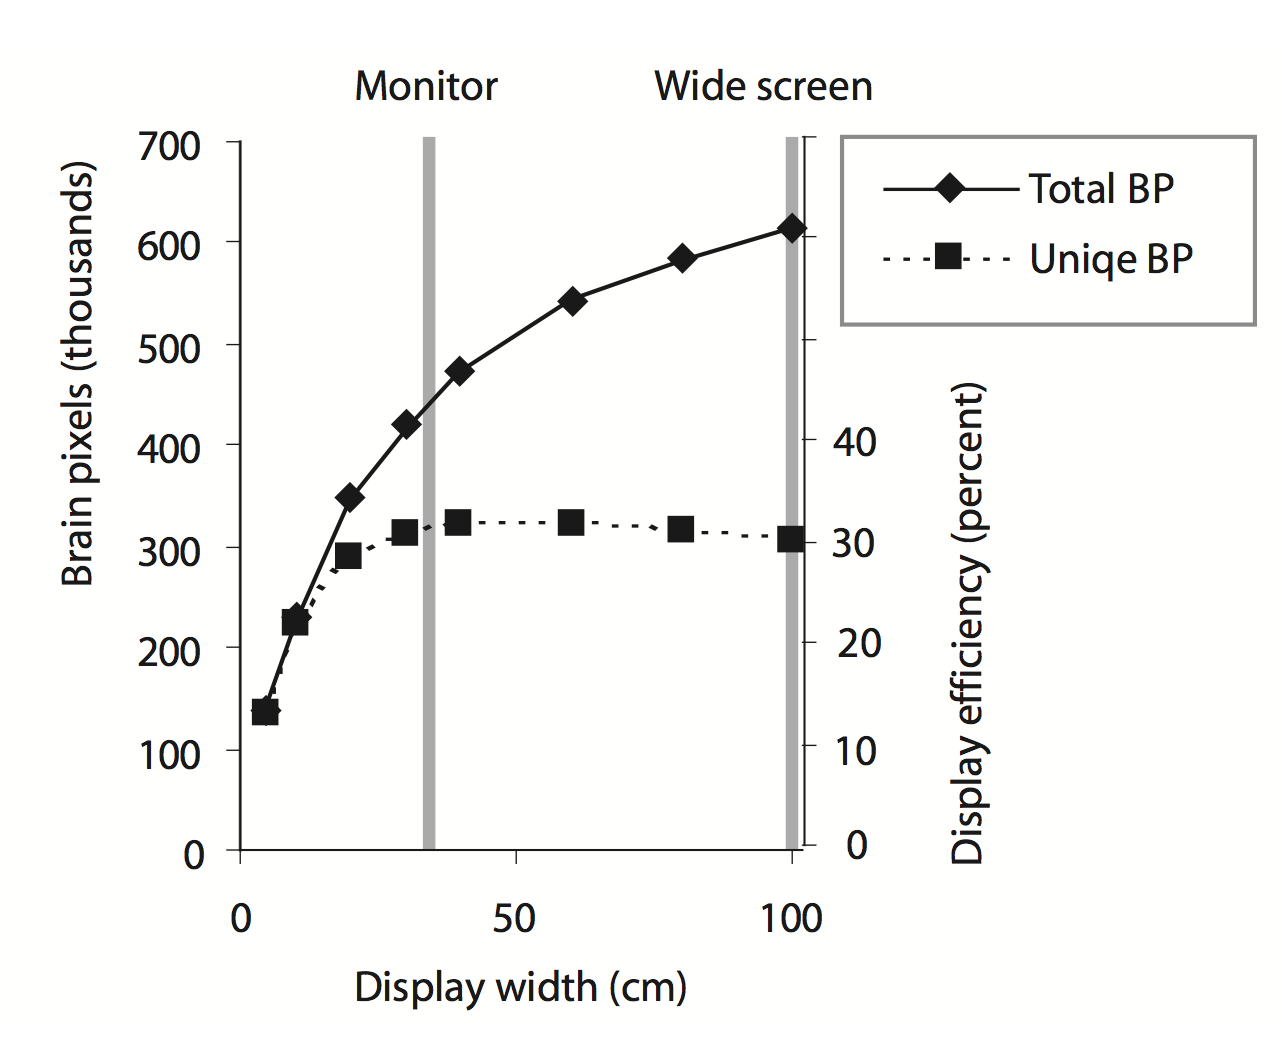
\includegraphics{src/images/DE}}
    \caption{Simulation of display efficiency by exposing the brain to a 1 mio. pixel screen. From \cite{Ware2012a}.}
    \label{fig:DE}
\end{figure}

This shows, that a monitor larger than 40cm wide are not increasing the display efficiency anymore. For large data sets this allows the conclusion that the perception of large data has a limit in the human perception. The current monitor size (which approximately is  40-50cm) is sufficient to respond to the number of USBP.

Talking of TBP  the human visual system is able to perceive 15mio pixels per eye\cite{Deering1998}. Assuming that the amount of perceivable pixels for two eyes is larger than 15mio pixels but smaller than 30mio pixels due to the overlap of the field of view the max. amount of perceivable pixels (pp) is:
\begin{math}
15 mio. \leq pp < 30 mio.
\end{math}

Nevertheless, the important question is not the amount of perceivable pixels but whether the data structure, patterns, trends and further information in the data can be perceived as the human brain is a pattern detection machine\cite{Ware2012a}. If we consider the brains ability to detect patterns aggregation methods for visualizations are not only tolerated but moreover recommended. Moreover, the main concern for visualization techniques should be the perception of patterns: trend, outliers, clusters. 
\par
In conclusion, human perception shows that visual scalability of techniques and monitor resolution are not important. The interesting question is whether tools integrate aggregation methods to outline patterns. \label{pattern}
Aggregation methods can either aggregate data inside the data set or inside the visualization. Examples for data set aggregation are calculated dimensions which joins multiple dimensions into a new one. Examples for visualization aggregation are clustered markers. The data set aggregation is discussed in section \ref{analytical} and visualization aggregation in section \ref{advancedmetaphor}.

\subsection{Analytical Techniques}\label{analytical}
Comparing the visualization techniques in \ref{vis} only few techniques scaled beyond 2 mio. pixels. Thus, the need for data reduction becomes obvious. In the literature \textit{data abstraction and aggregation} are well know techniques for data reduction\cite{FerreiradeOliveira2003,Aigner2011, Keim2005}. There exist two ways to data reduction: to reduce data horizontally or vertically. 
Vertical data reduction describes the process of removing data rows whereas horizontal data reduction is used for dimensionality reduction. 
\begin{figure}[H]
    \centering
        \scalebox{.1}{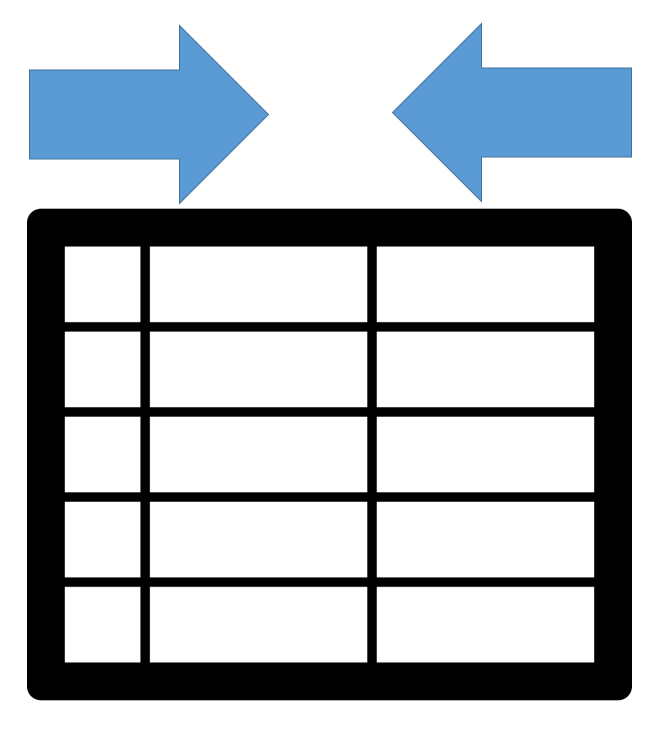
\includegraphics{src/images/dimreduce}}
    \caption{Horizontal Data Reduction}
    \label{fig:my_label}
\end{figure}

\begin{figure}[H]
    \centering
        \scalebox{.1}{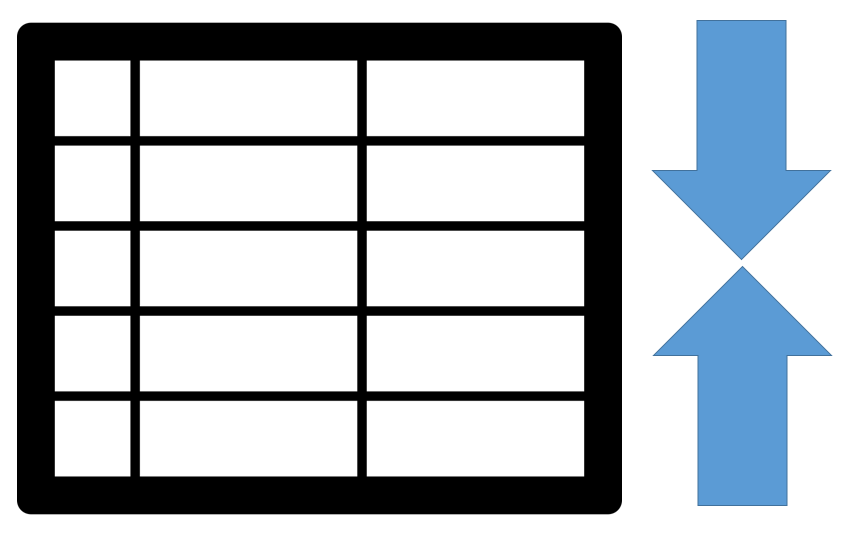
\includegraphics{src/images/aggregation}}
    \caption{Vertical Data Reduction}
    \label{fig:my_label}
\end{figure}

\subsubsection{Vertical Data Reduction}
One way to decrease the size of large or huge data sets is to remove data rows. This section lists several data removal techniques. 
%One important issue for every technique is the question which data to keep and which data to remove. The disadvantage of data reduction is the information loss.
\textbf{Sampling \& Filtering: }\label{sampling}\label{filtering}
Sampling describes a strategy to reduce data by creating a subset of the original data. Thereby, sampling is scalable, reduces clutter, preserves information of the kept data as well as patterns and trends\cite{PiringerHarald2011}. Still, sampling may eliminate outliers or single data items and does not provide any guarantee to avoid visual overlap. \\*
Filtering is a method to reduce data by some specific criteria. In visualization filtering often is based on user input such as dynamic query sliders in the frontend. In the backend filtering can also applied to define data extracts. In both cases filtering can support the user in excluding task-irrelevant data portions and unlike sampling filtering may be appropriate to detect outliers. However, as filtering is based on the exclusion of irrelevant attributes it does not guarantee a specific target size of the data set. In some cases the target size might still be too large. Moreover, filtering also does not secure the discrimination of distinct data items\cite{PiringerHarald2011}.\\*
\textbf{Aggregation: }\label{aggregation}
Aggregation describes the process of grouping similar data items together. Hierarchical aggregation builds aggregated data items by forming a tree structure and collapsing the children of a tree\cite{elmqvist2010hierarchical}. Binned aggregation divides data into adjacent bins and combines them for aggregation\cite{Liu2013}. Pixel-aware aggregation clusters pixels according to their screen coordinates\cite{li2016polyspector}. M4 aggregation compresses time series data into a set of equidistant time spans\cite{jugel2014m4}.
As time-oriented data has specific characteristics analytical methods have to consider these peculiarities. One way to reduce data size with respect to the time-specific characteristics is temporal aggregation. Hereby, data is aggregated according to the time unit (day, month, year) in temporal hierarchy levels. Examples for temporal aggregation are hierarchical axis \cite{Chung2014} which enable to navigate in time. 
\\*
\textbf{Temporal Data Abstraction: }
Temporal Data Abstraction\cite{Aigner2011} reduces the number of data rows by focusing on relevant concepts, patterns, shapes over time and neglecting irrelevant details. Clusters and summery statistics\cite{PiringerHarald2011} are typical examples for data abstraction. In the context of time-oriented data  However, the authors found a trade-off between abstraction and accuracy: with low abstraction and a high accuracy there exists the problem of cluttering. 
One way to implement temporal data abstraction is to use natural language processing in visualization tools. The tool \textit{Answerrocket} implemented an NLP-Approach connected with visualization. Another way to achieve data abstraction are unsupervised machine learning methods, such as clustering.
Clustering as defined in the user tasks \ref{tasks} as \textbf{T2} has the advantage of reducing visual clutter by displaying the natural groups of the data instead of every single data item. It also preserves pattern and outlier if the similarity measure is appropriate.\\*
Temporal Data Abstraction in tools can be implemented by any method which keeps the characteristic shape and removes data points. \\*

Other ways to reduce data vertically are binning and pivoting. We will not explain them here in detail as they treat continuous and hierarchical data sets which are beyond our scope. 

\subsubsection{Horizontal Data Reduction}
Besides data removal data size can be reduced by decreasing data dimensionality. Since business data often is multi-dimensional but visualization techniques are limited in the number of attributes dimensionality reduction is a way to process data sets in a way that they can be displayed by visualization techniques. 
\textbf{Dimensional Reduction: }Common dimensionality reduction techniques are Principal Component Analysis (PCA)\cite{Aigner2008}, K-Means Clustering\cite{AllenHamilton}, Multi-Dimensional Scaling or  Self-Organizing Maps\cite{PiringerHarald2011}. The advantage is that they keep the distance between two points after the projection. Thus, anomalies can be detected and the user can be supported in \textbf{T6}.\\* 
\textbf{Calculated Dimensions: }Dimensions also can be reduced by aggregated dimensions also known as calculated dimensions. Instead of visualizing the original dimensions aggregated dimensions are visualized and thus, multiple dimensions can be combined.\\*

In short, data reduction techniques such as horizontal and vertical data reduction condense  data sets in way to fit data sets on the screen and overcome the problem of visual clutter. With data reduction non-scalable visualization techniques can be used. 

% \subsubsection{Data Modeling}
% Next do data reduction techniques \textit{data modeling} techniques are an important feature for tools. They enable the user to find patterns in the data and thus, support the user in the user tasks \textbf{T2, T5, T6}. Data Modeling covers clustering, classification, network modeling and predictive modeling\cite{Zhanga}. 

\subsubsection{Pattern Search}\label{patternsearch}
Besides data reduction, pattern search is an important feature in navigating in a large data set. Given a defined pattern similar patterns are retrieved. One implementation of pattern search are \textit{Timeboxes}\cite{Buono}. With timeboxes the user can drag out a rectangle which defines the pattern. Then similar patterns are queried and retrieved. That is why pattern search supports the user in the user tasks \textbf{T1} and \textbf{T7} by detecting regions of interest and supporting in navigation. In large data sets pattern search is required more than ever as the human perception is not able to perceive patterns anymore.


\subsection{Advanced Visual Metaphors}{advancedmetaphor}
Another way to implement aggregation (\ref{pattern}) are advanced visual metaphors. Visual metaphors define how data is mapped to geometric primitives. Thereby, the mapping function influences visual scalability. The visual metaphor of pixel-oriented techniques maps each data item to one pixel. Hence, the maximum number of displayed pixels is equal to the number of screen pixels. The visual metaphor of bar charts  arrange data items as bars along the monitor width ($w$). Thus, if each bar would have the width of one pixel, a bar chart could only visualize  $w$ data items. Thus, the visual metaphor limits how many data items can be showed at most. Advanced visual metaphors can enhance the scalability of visualization techniques\cite{Eick2002}. \\*
 \textbf{Multi-resolution:} \label{multi-resolution} one way to improve visual metaphors are \textbf{multi-resolution} metaphors\cite{Keim2005}. The idea of multi-resolution is to assign relevance to each data point and aggregate them. Less relevant data are condensed to larger clusters while more relevant data have smaller clusters. Then the clusters are mapped to the screen space. Thus, the resolution denotes the ratio of data items compared to screen pixels. Pixel-oriented techniques have a resolution of 1:1 as they map one data item to one pixel. 
 \begin{figure}
     \centering
     \scalebox{0.5}{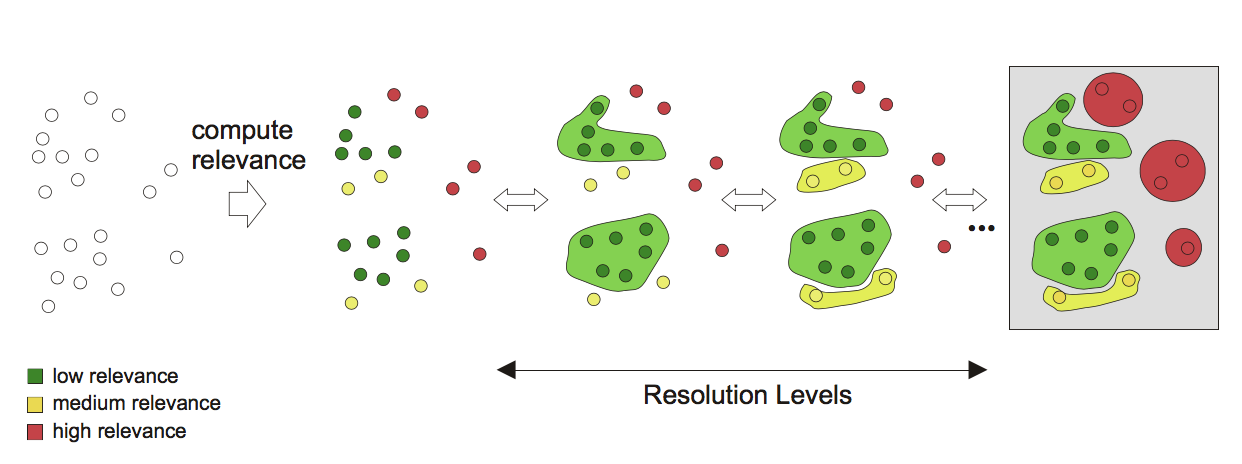
\includegraphics{src/images/multi-resolution}}
     \caption{\textit{Multi-Resolution: }data items are grouped with variying granularity depending on their relevance. From \cite{Keim2005}}
     \label{multi-resolution}
 \end{figure}
 In a multi-resolution visualization the resolution is usually less granular at the \textit{Overview-Level} and more granular at the \textit{Detail-Level}. \textit{CircleView} is one visualization technique with a multi-resolution metaphor. Multi-resolution is one important aspect for visualization tools to improve visual scalability.\\*
\textbf{Aggregation Markers:}\label{aggregationmarkers} A different approach for advanced visual metaphors are aggregation markers which were already mentioned by Shneiderman\cite{Shneiderman2008}. He proposed to extend the Information Seeking Mantra\cite{Shneiderman1996} with point clustering which he called aggregation markers. Point clustering groups a larger set of data points onto a smaller set in the 2D-plane\cite{Morrison2014}. This process decreases the visual overlap of data points and thus, increases the perception of large data sets. Moreover, point clustering accelerates the rendering process by first rendering the data clusters  and later loading more detailed data items. This incremental loading fulfills user satisfaction by shorter response times.\\*
In contrast to data reduction methods advanced visual metaphors are not actually decreasing data size. They only decrease the \textit{perceived data volume} and keep the actual data volume. This differentiates methods like multi-resolution and aggregation markers from methods like data reduction. 


\subsection{Need for Interaction Techniques}
Interaction Techniques describe how the user can interact with the data. In this section interaction techniques for large data sets are discussed and how they can enhance scalability. As discussed in \ref{problems} challenges in visualization are pixel overlap, limited screen space, identifying a region of interest and navigation. Interaction technique can overcome these problems. 
\par
Overlap can be eliminated by filtering and zooming as filters and zoom reduce the displayed data and hence, minimize the overlap. \\*
\textbf{Filtering:} With filters a set of variables can be selected and the visualization is only showing the respecting variables. The excluded data items are kept in memory.
One way of filtering are dynamic queries. They provide a filter-mechanism by multiple widgets, such as sliders or input fields\cite{Hochheiser2004,Shneiderman2008,Aigner2011}. A specific dynamic query for time-oriented data are time-boxes. These boxes are rectangular selection areas which are drawn by the user. The tool then only displays values with a similar pattern to the pattern in the time-boxes.\\*
\textbf{Zooming} is the way of drilling down into a data set to a lower level of detail. The user focus is shifted from the \textit{Overview}-Level to a \textit{Detail-Level} where the displayed data is reduced and thus, overlap decreased. One special way of zooming is semantic zooming\cite{boulos2003use}. Instead of zooming multiple linked views are preferred for a higher number of displayed object. This will be discussed in \ref{zoomingVsmultiple}. 
\par

The limited screen space can be enhanced by \textit{interactive distortion techniques}\cite{mackinlay1991perspective}.
The main idea of distortion techniques is to present more relevant data enlarged in the user focus while less relevant data are shown at the context in a smaller presentation. Distortion technique are not providing additional pixel to the existing screen pixels but they enhance the screen space metaphor by prioritizing screen pixels.
Examples for distortion techniques are \textit{Bifocal Displays}\cite{Spence1982}, \textit{Fish-eye Views} and \textit{Perspective walls\cite{Keim2005}, \cite{mackinlay1991perspective}}.\\*
All distortion techniques transform the undistorted 2D space by a mathematical function and bring more relevant data points to the focus.\\* 
\textbf{Bifocal Displays} bend the space with a linear function.\\*
\textbf{Fish-eye Views} (also known as Table and Magnification Lense) apply a power function and\\*
\textbf{Perspective walls} distort the space by applying both linear and power function. Thus, a 3D-representation is created which exists of 3 walls. The front wall shows details and the two side walls provide context. Perspective walls is one method to provide \textbf{Focus + Context} and Navigation in large data sets.
\begin{figure}[H]
    \centering
        \scalebox{.25}{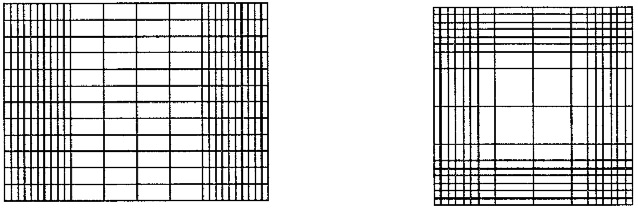
\includegraphics{src/images/f06b}}
    \caption{Bifocal Displays: distortion by linear function. From \cite{Stroe1999}.}
    \label{fig:bifocal}
\end{figure}

\begin{figure}[H]
    \centering
        \scalebox{.25}{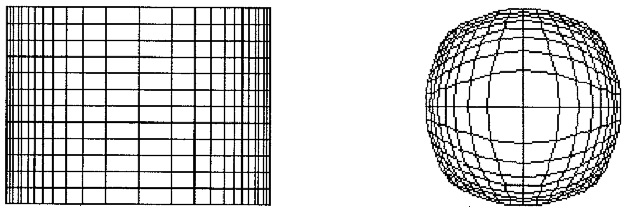
\includegraphics{src/images/f11c}}
    \caption{Fish-eye views:  distortion by a power function with an odd exponent \cite{Stroe1999}.}
    \label{fig:fisheye}
\end{figure}

\begin{figure}[H]
    \centering
        \scalebox{.25}{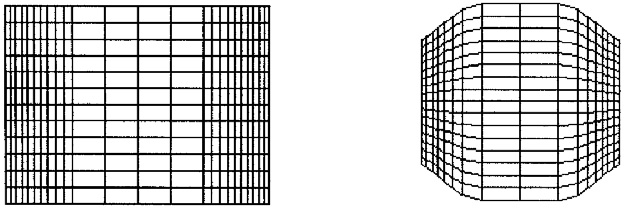
\includegraphics{src/images/f10b}}
    \caption{Perspective Walls: distortion by a half linear and half power function From \cite{Stroe1999}.}
    \label{fig:perspectivewall}
\end{figure}
Distortion techniques are good in finding outliers. One disadvantage is that the user might loose the context.
\par

\label{navigation}
In close relation to interaction techniques stand appropriate \textit{interactive navigation techniques} to navigate inside the data set such as linked views and information murals, also known as navigational maps\cite{Jerding1998}. With linked views the user can see different level of detail on one glance and navigate in different level of detail with navigational maps. Navigation also helps in finding a region of interest.\\*. The differentiation between navigation and interaction techniques is not selective.
\label{zoomingVsmultiple}
Ware\cite{Ware2012} showed that zooming is an easy-to-use-tool for a small amount of items. However, if the user needs to keep three items or more in its visual working memory multiple windows are more effective than zooming. Thus, displaying large time-oriented data requires a layout with multiple simultaneous views if the number of data objects exceeds three items. Multiple coordinated views are called linked views. Often, linked views are combined with Brushing. \\*

\textbf{Brushing \& Linking: }The user can select data items on the screen(Brushing) and the respective items are highlighted in every connected window (Linking) which is also known as coordinated window. Therefore, lasso, rubber-band or rectangular selection enables the user to select groups of data items\cite{tegarden1999, Aigner2011}. Brushing \& Linking is one way to achieve \textit{Focus + Context} but it also supports the user by the user task \textbf{T3} as similar items are highlighted. Moreover, in the context of time-oriented data a typical brushing activity is the selection of an smaller time-span to see more details during this period of time. 
\\*

\begin{figure}[H]
    \centering
        \scalebox{.3}{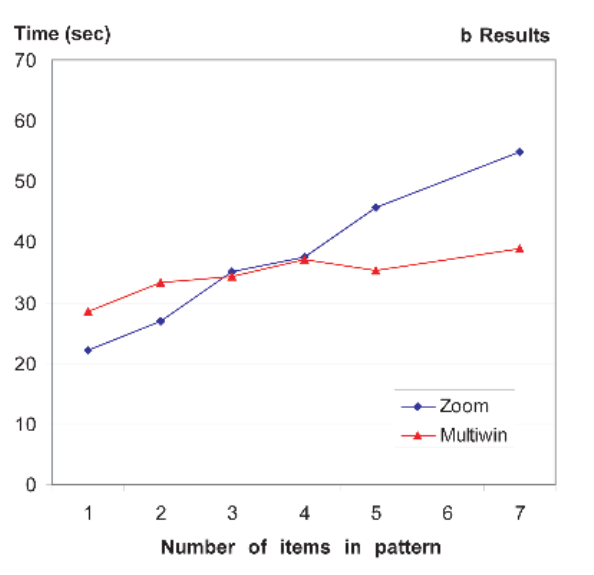
\includegraphics{src/images/zoomVSmultiWindow}}
    \caption{Measured task performance of zooming compared to multiple windows. \cite{Ware2012a}}
    \label{fig:my_label}
\end{figure}

Another navigation technique for large data sets are \textbf{navigational maps}.\\*
\textbf{Navigational Maps: } display the complete data set next to other linked views as a miniature version in a separate window. With this method, the user can as well see the data set in detail as well keep the context and navigate through the data set.\\*
\textbf{Search: }\label{search} Besides navigational maps \textit{Searching} is an approach in querying and retrieving one specific data point. Searching uses natural language processing (NLP). As data set searching can include solutions from the text input at the front-end or it also can consider solutions from the data points - displayed in the visualization. The second case is recommended for large data as the number of data points is difficult to overview.
\par

The discussed interaction techniques are only a subset of available interaction techniques. We focused on interaction styles which can solve the problems of large data visualization and thus enhance visual scalability\cite{Tegarden1999}. Hereby, we assume that interaction is in responsibility of the visualization tools.


\begin{table}[H]

    \begin{tabular}{|l| l l l|}
        \hline
            &                   & 1 & 2\\
        \hline
            &                   & \begin{turn}{90} Multi-Resolution\end{turn}   & \begin{turn}{90} Aggregation\end{turn}\\
        \hline
        A   & avoids overlap    & \checkmark                                    &\\
        B   & keeps spatial information     & x                                 &\\
        C   & can be localised  & \checkmark                                    &\\
        D   & is scalable       & \checkmark                                    &\\
        E   & is adjustable     & x                                             &\\
        F   & can show point/ line attribute    & x                             &\\
        G   & can discriminate points/ lines    & x                             &\\
        H   & can see overlap density           & x                             &\\
        \hline
    \end{tabular}
\end{table}



\section{Visual Scalability 2.0}
After our analysis of the limiting factors for displaying large data sets we come to the conclusion that the limitation by human perception is more restrictive than the limitation by different visualization techniques. The question is \textit{not} how many pixel can be displayed by a visualization technique but whether the visualization technique allows to perceive patterns. This is achieved by the use of \textit{appropriate visual metaphors} and \textit{data reduction methods}. Data reduction methods can aggregate overlapping data items to cluster by either mapping data density to color or by displaying the mean and the range of data. Visual Metaphors include techniques such as multi-resolution and thus, enhance the number of pixels which can be displayed. Data and dimension reduction reduces the number of data items which needs to be displayed. Thus, even non-scalable visualization techniques can display the reduced data. 

\subsection{Success Criteria for large scale data visualization}\label{success}
Bringing all findings together, the important factors for the visualization of large data sets to support decision-making are the following: 
\begin{enumerate}[noitemsep]
\item How are advanced visualization techniques integrated? 
\item How is data reduction achieved? 
\item How are aggregation metaphors implemented? 
\item How are interaction techniques supported?
\end{enumerate}

Visualization tools need to offer solutions to these questions for a successful visualization of large data sets. Thus, we propose the following success criteria for large data visualizations and define a best possible implementation. This definition will be equivalent to the best score for completeness of the scoring model in chapter \ref{chap:Tools}.
\begin{enumerate} [noitemsep]
\item Analytical Techniques 
\begin{enumerate}
    \item The tool offers horizontal data reduction.
    \begin{itemize}
        \item Let $k$ be the desired number of dimensions. A data set can be reduced to $k$ dimensions. The visualization takes $k$ dimensions as input.
        \item Dimensions can be aggregated and saved as a new dimension.
    \end{itemize}
    \item The tool offers vertical data reduction.
    \begin{itemize}
        \item Data sets can be reduced by omitting rows.
        \item Filter are offered to interactively reduce the number of showed data items.
        \item Data points can be removed from data set. 
        \item Relevance can be assigned to data points so that important data points can be kept and less relevant data points removed.
        \item Data items can be clustered and saved.  
    \end{itemize}
\end{enumerate}


\item Visualization Techniques
\begin{enumerate}
\item The tool offers all possible visualization techniques.
\item Every visualization technique can cluster or aggregate data items.
\item Every visualization technique can use multi-resolution.
\end{enumerate}

\item Interaction Techniques
\begin{enumerate}
\item The tool offers the drill-down functions zoom and filter for every visualization.
\item The tool offers the distortion techniques fish-eye, perspective wall, bifocal display for every visualization.
\item The tool offers the navigation techniques navigational maps, coordinated windows, searching for every visualization.
\end{enumerate}

\end{enumerate}

In the next chapter we will compare different state-of-the art tools regarding this success criteria for large data visualization.


\chapter{Investigation of Visualization Tools using a Feature Classification Scheme}
\label{chap:Tools}

In this section we analyze selected visualization tools which are used in business and their ability to visualize large time-oriented data. Therefore, we developed a classification scheme which is based on the collected success criteria of chapter \ref{chap:BIV}. \\*
As discussed in chapter \ref{chap:BIV} visualization tools need to provide scalable visualization techniques or the ability to extend the tool with custom visualizations. Moreover, Interaction and distortion techniques are necessary to improve scalability. Analytical methods reduce the amount of data vertically and horizontally. 
\section{Selection of Tools}\label{tool:selection}
ADV in business context requires software that is able to scale visualization in an "effective manner"\cite{Russom2011}. Offering ADV techniques, parameterization, interaction and analytical methods such as data abstraction\cite{Tegarden1999,Aigner2011,Eick2002,Zhanga} are core functions of ADV software. \\*
\textbf{The Role of APIs}
Commercial software tends to need more time for the development and integration of advanced visualization for large data\cite{Zhanga, Simon2014}. To bridge the gap, vendors started to offer a bunch of APIs to expand the visualization functions. 
% data load for BigData: 
\textbf{Software not included in this work}
As the goal of this work is to compare visualization tools in business we only consider software which is 
\begin{enumerate}
    \item generic: not specialized to one domain
    \item integrates visualization features
\end{enumerate}

Furthermore, the software needs visualization features, the ability to present time-dependent data. Software with one of the following items is intentionally not considered: 
\begin{enumerate}
    \item Software that only presents one-dimensional data. 
    \item Software that is specialized to data mining.
\end{enumerate}

Based on the Magic Quadrant for Business Intelligence and Analytics Platforms 2017 \cite{Sallam2017} Qlik, Tableau and Microsoft are the leading visionaries of BI Vendors. \cite{ITCentralStation} as a crowdsourcing recommendation platform for BI tools ranked Tableau, Qlik, Oracle, Microsoft Power BI and IBM Cognos on the first five places. Nevertheless, marketrelevance reports from Gartner, Forrester, Barc and other so called "research and advisory companies" usually do not publish a detailed scoring model. Thus, the ranking might not be appropriate to our needs.

Eventhough, Qlik, Tableau and Power BI are ranked as BI tools they can call themselves visualization tools. 
Thus, we chose the tools: Power BI, Tableau and Qlik Sense (QS).\\*
Moreover, we added d3.js as this javascript library is open-source, state-of-the art in visualization and offers a wide range of visualization possibilities.

Even though the selection of the tools is not exhaustive, we believe that the reviewed products represent the state-of-the art and provide the table of different tools which was used for chosing the remaining 5 tools in the appendix.

\subsection*{Qlik Sense}
Qliktech was founded in 1993 with the goal to "mimic how the brain works."\cite{qlikHistory}. They offer five products(QS, QS Cloud, QlikView, QlikView NPrinting, Qlik DataMarket) and the Qlik Analytics platform. QS 1.0 was released in September 2014 for visual analytics. 
\todo{evlt. raus}
It offers functions such as Smart Data Load which allows to load large data from different data sources.

\subsection*{Power BI}
Microsoft Power BI came alive in ...\todo{datum einfügen}. It is made up of six main components: 
\begin{enumerate}
    \item Power Query: Data Mesh-up tool
    \item Power Pivot: Data Modelling Tool
    \item Power View: Data Visualization Tool
    \item Power Map: 3D Geo-spatial data visualization tool
    \item Power BI Desktop: Reporting Tool 
\end{enumerate}
These components can be combined for interactive data analysis. In our work we will focus on the data visualization tool: Power View. We will briefly discuss Power Pivot in the context of database metrics. 

\subsection*{d3.js}
d3.js is a javascript library used for visualization. It visualizes data based on SVG, HTML5 and CSS and binds data to existing web elements in alignment with the Document Object Model (DOM).  Data Handling is managed by the underlying data source, data modeling can be handled by other javascript libraries such as node.js. A good overview how d3.js works is given in \cite{Meeks}. 
We chose d3.js as it is a data visualization tool with interaction. As it is free it becomes an alternative to commercial tools.

\subsection*{R}
R is a free and opensource language for statistical computing and graphics. Its modular structure consisting of many packages makes R highly extendable\cite{R}. Some packages enable the user to do analytics with R, others support different visualization techniques. Usually those packages also support interaction except the user additionally uses other libraries such as plot\_ly() or Shiny. Both of them are frameworks which combine R graphics with interaction techniques. Besides of that some packages offer interaction techniques, e.g. dygraphs(), while others do not. Thus, our classification scheme is only valid combined with specific packages.
There exists many packages which treat time-series data, e.g. \textit{zoo} and \textit{dygraphs} treat time-series. Large data sets are handled in \textit{bigvis}.

\section{Scalability of visualization tools}\label{tool:scalability}
The scalability of visualization tools is measured by the \text{visualization characteristics} and the \textit{database metrics}. Moreover, as discussed in \ref{chap:BIV} important features are interaction techniques and analytical methods. 

\subsection{Database metrics}
According to Eick visual scalability is not only determined by the visualization characteristics but also by the database metrics. Eick defined database metrics as the size of the database which can be handled by tools\cite{Eick2002}. One possibility to measure the database size are the number of lines which can be load into the tool and the limitations on visualizations in the number of rows.\\*\\*
While \textbf{Tableau} and \textbf{Power BI} have no limitations how many data can be loaded, \textbf{QS} inherits the data load limitations of Qlik View: A QS document cannot have more than 2,147,483,648 distinct values in one field. This limitation still allows Qlik to handle large and huge data sets according to our definition. Moreover, 2 billion data points exceed the limit of screen pixels. But nevertheless, QS is outperformed by Tableau and Power BI in this particular case.
\\*\\*
In context of visualization the number of rows which are loaded into a visualization is a determining factor for scalability. For large data the user expects to load all data he wants the tool to load. However, some tools limit the initial number of rows and the user has to write additional code. This effects the easy-of-use negatively.
QS limits the initial fetch to 10.000 but gives the opportunity to fetch more data if needed. \textbf{Power BI} and \textbf{Tableau} currently have no limit for rows in visualization.
Again QS stays behind Tableau and Power BI.
d3.js 

\subsection*{More than database metrics}
Nowadays, data management shifted from importing csv-files or Excel Spreadsheets to storing data sets in technologies such as clouds or databases. 
Therefore, most of the visualization tools provide data engines, an underlying software component which manages the data. Thus, the tool performance depends at the following factors:
\begin{enumerate}
    \item Hardware Resources
    \item the underlying engine
    \item perceived performance 
\end{enumerate}
In our understanding of visual scalability Eicks definition of database metrics needs to be adjusted in a way that it meets the characteristics of tools today. Thus, we expand \textbf{database metrics} by the ability to integrate data storage.

\textbf{In-memory versus Real Time Connection}
In-memory techniques store their data inside the RAM while real time technologies work directly on the database.
With large data sets in-memory technologies might not be feasible. Eventhough, working in-memory is faster than working directly at the database. With a smaller subset of large databases working in-memory might be the better option. 
\textbf{QS} data engine (QIX Engine) and \textbf{Power BI} use in-memory columnbased technology. While the data engine processes calculation the RAM may be temporarily allocated. Thus, QS is limited by the primary memory of the computer. \textbf{Power BI} also connects live to clouds and on premises similar to \textbf{Tableaus} Data Engine which is designed to work live on the database. At Tableau data extracts can be created to work in-memory. The limits for data extracts are not published but Tableau Public, the free version of Tableau, recently extended the limit of 1 mio. rows to 10 mio. rows in-memory. 
For working with large data sets Tableau again outperformed QS and Power BI.\\*
\textbf{Connection to multiple data sources}
With large data sets data is distributed about several places. The ability to connect to multiple databases impacts the scalability. All of the tools can connect to multiple data sources. In future work, a performance review for the connection of the tools to multiple data sources is recommended.\\*
\textbf{Incremental Loading}
With large data sets tools might be overstrained with loading the whole data sets at once. Strategies to tackle this problem are incremental load. \textbf{QS} uses a custom data model called .QVD files. In .QVD files data is highly compressed and allows incremental loading. Tableau allows the incremental refresh of data extracts which adds only new rows to the extract. Power BI does not offer the option of incremental loading. 
\textbf{Further Aspects}
Scalability of tools can also be measured in terms of users and delivery which goes beyond our scope.




\subsection{Visualization Characteristics}
In the context of \textit{visualization characteristics} QS, Tableau, Power BI and d3.js have been compared regarding \textit{Visualization Techniques, Analytical Techniques and Interaction Techniques}. 

\subsection*{Qlik Sense}

\subsubsection*{Visualization Techniques}
QS offers 8 built-in visualization techniques: bar charts, line charts, pie charts, scatterplots, treemap, maps, combi charts and gauge charts. If an additional technique is wanted the user can either use one of the community's self-made extensions or he can build his own visualization extension with \textit{javascript} and \textit{QEXT} files\cite{qlikWorkbench}. QS provides an extension template which supports the user in writing its extensions. Moreover, Qlik provides 20 high-level-APIs which supports the user in writing a custom extension. However, the user needs to know javascript and html\cite{qlikVisExtensions}, as well as QS own QEXT-language. \\*
Out of the QS standard repertoire non of the visualization technique corresponds to the studied visualization techniques of chapter \ref{chap:BIV}. With d3.js it would be possible to build these visualization techniques and integrate them in QS. 
The embedding of javascript also allows \textbf{Aggregation} in terms of multi-resolution and the use of aggregation markers. However, this again requires coding-skills. 

In the field of built-in-aggregation markers QS offers data aggregation for one chart type: the scatterplot. Hereby, large data is aggregated by aggregation markers. When the scatterplot is shown at an overview level accumulated data points are represented by squares. The color shows the data items density. The darker the square the denser the data\cite{qlikScatter}. With the so called \textit{Smart Data compression} Qlik starts to consider large data amounts. However, offering Smart Data Compression only for one technique Qlik stays behind the present day requirements.


\begin{figure}[H]
    \centering
    \subfloat[QS]{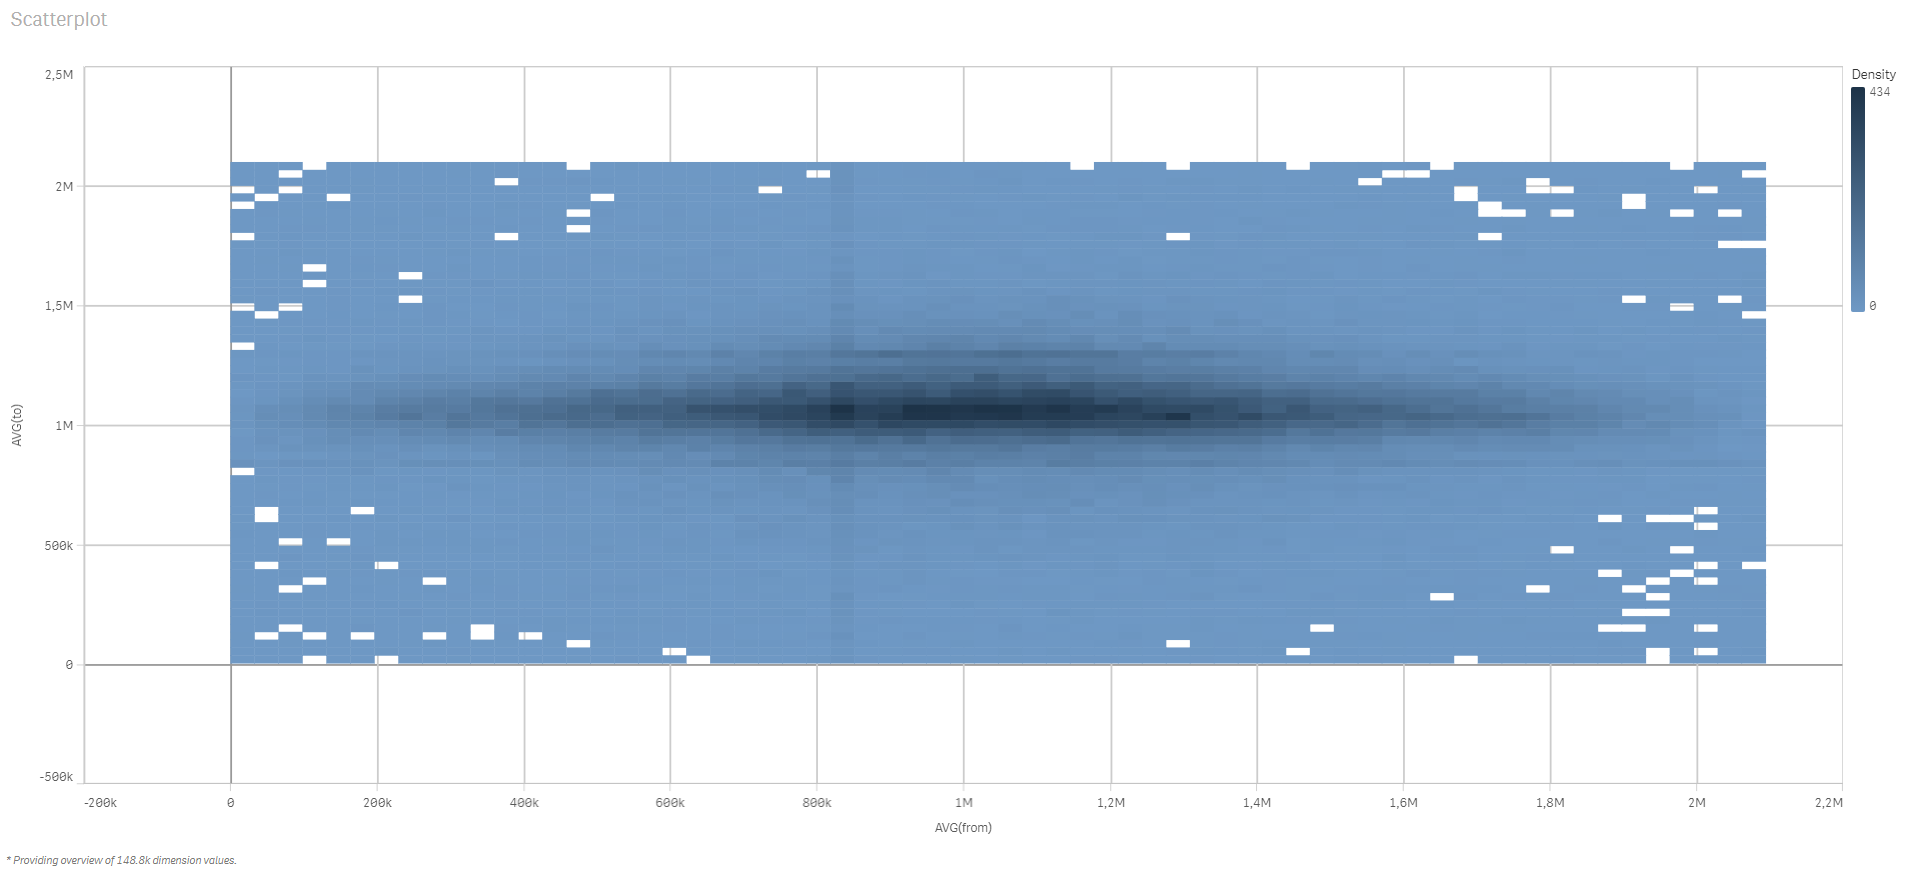
\includegraphics[width=6cm]{src/images/SmartDataCompression}}
    \caption{Smart Data Compression (left): Overview level which shows aggregated data points by squares and color and changes the shape if zoomed in}
    \label{fig:smartdatacompression}
\end{figure}

\begin{figure}[H]
    \centering
    \subfloat[Sparse Area]{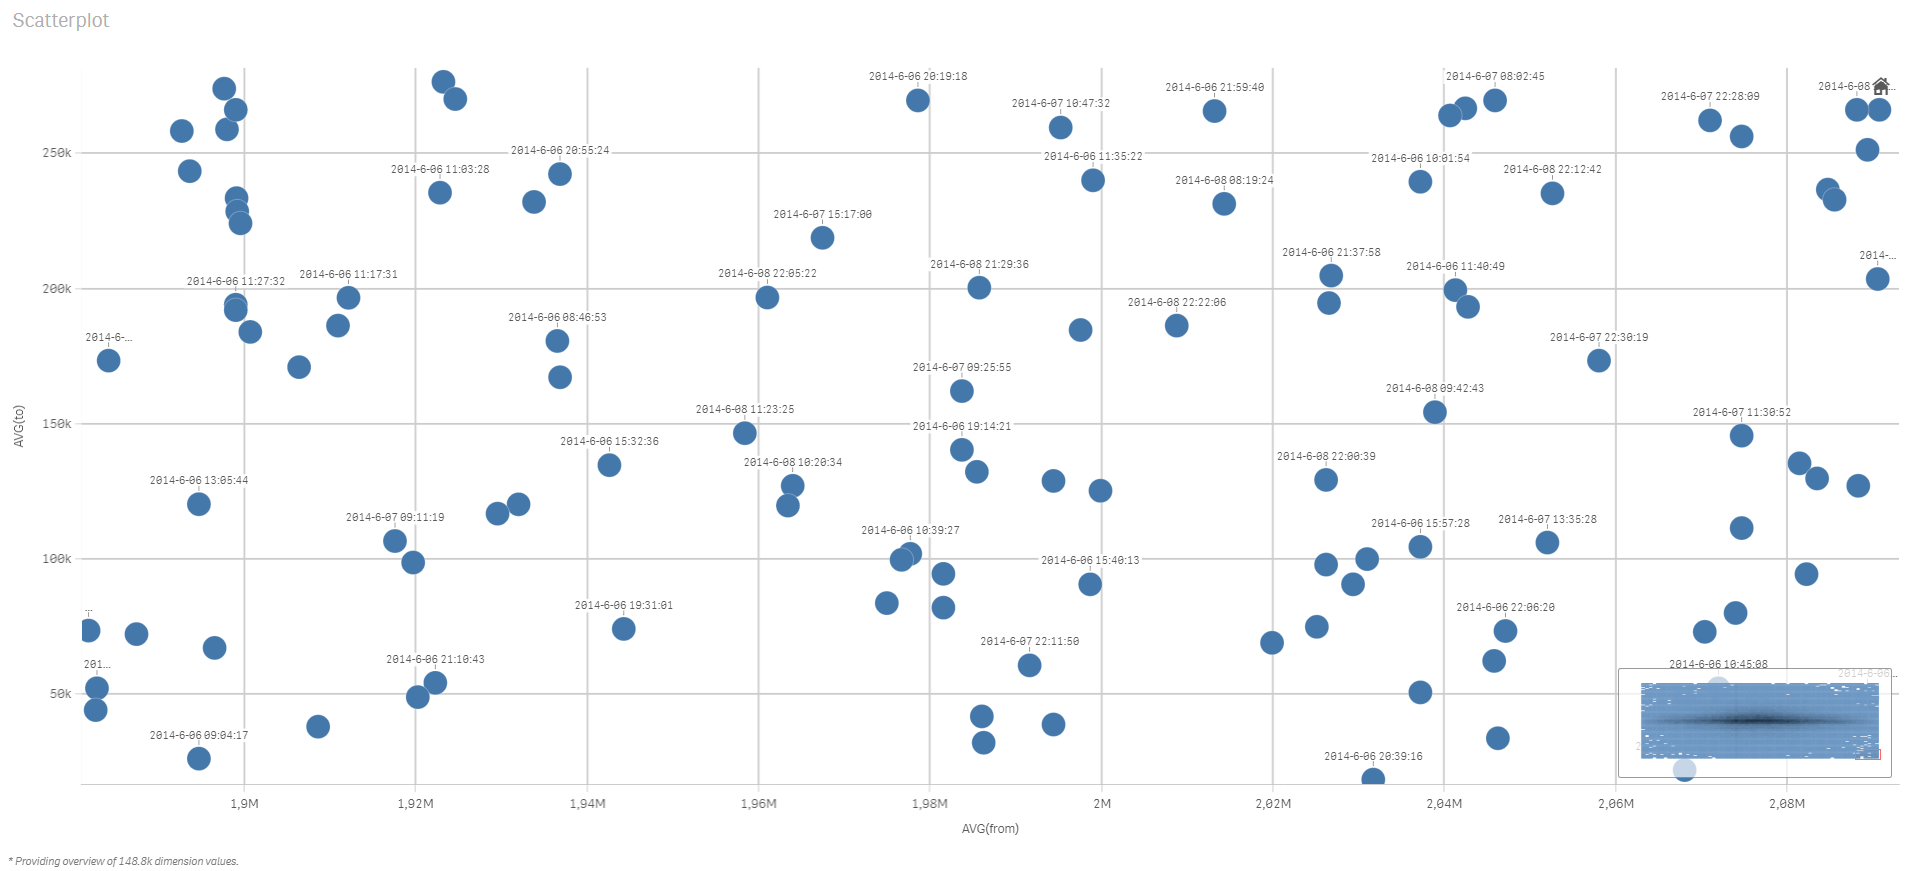
\includegraphics[width=6cm]{src/images/SmartDataCompressionI}}
    \qquad
    \subfloat[Dense Area]{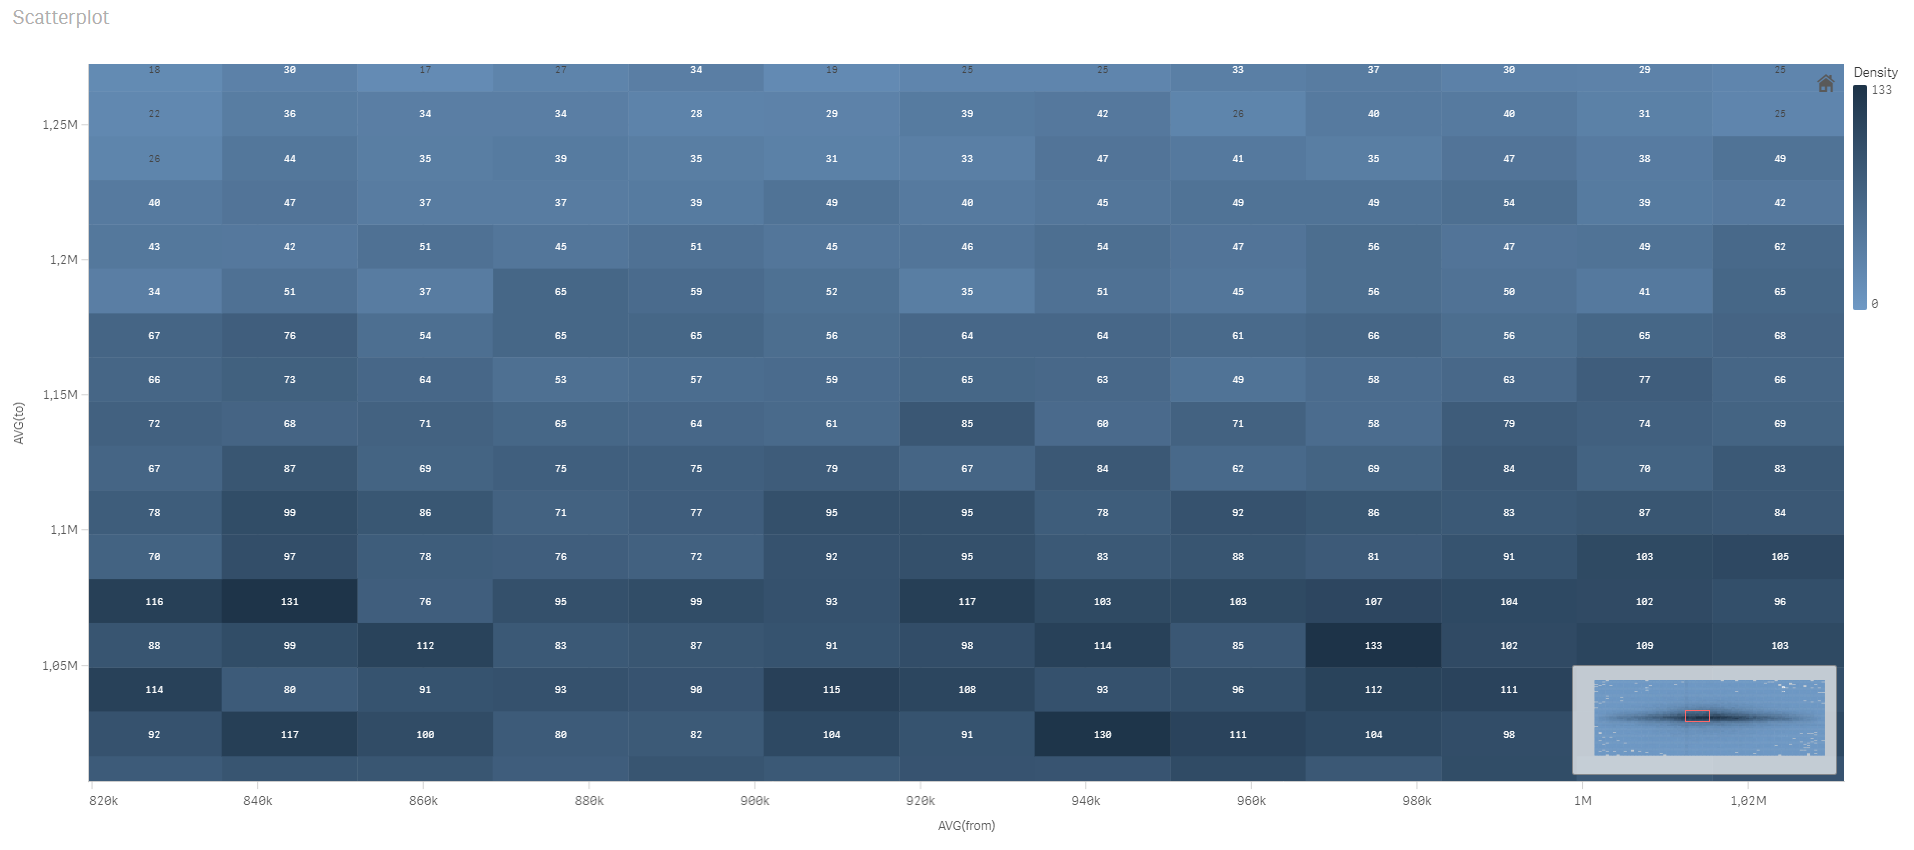
\includegraphics[width=6cm]{src/images/SmartDataCompressionII}}
    \caption{Smart Data Compression: Detail level}
    \label{fig:smartdatacompression}
\end{figure}

\subsubsection*{Analytics}
Data reduction is part of QS Server. With dynamic data reduction rows can be hidden for a group of users. Thus, data size is decreased. Internally, .QVD files compress data. But, the user cannot reduce data size based on an interactive selection inside the dashboard. In this case, the user could select a group of data and decide whether he wants to keep only the selected data. 
QS implements \textbf{Aggregation} with aggregation-functions. These use QS specific set expressions and range from basic statistical functions (min,avg,max) over financial functions, to advanced statistical functions(linear regression, correlation). With these aggregation functions QS offers some analytical methods. Yet, QS has no integration to an analytical program.
\subsubsection*{Interaction}
To allow a focus + context view QS offers navigational maps\cite{beard1990navigational} which come as navigational slider in which a miniature version of the whole data set\cite{beard1990navigational} is shown. 
Filters can be applied by making selections or dragging a filter inside the visualization\cite{qlikSheet}  and all views then are adapted to the current selection. Thus, QS offers Brushing + Linking. An additional linking-feature are \textit{master items}\cite{qlikChangeData}, which allow the user to change properties for all master items at once.
For details the user can search QS with Smart Search in which the dimensions, measures and metadata is searched and visualizations ,tables and KPIs are displayed\cite{qlikSmart}.  


\subsection*{Tableau}
The Tableau approach to large data visualization is \textit{extract data first, then visualize}. This approach is manifested in the fact, that some functionalities in Tableau are only available for data extracts. Count distinct, offline access and incremental refresh are these features.
Tableau published a guideline "Best Practises for Designing Efficient Tableau Workbooks" in which they recommend of showing the highest aggregation level first and show only a selection of records. This approach basically implements Shneidermans \textit{Overview first, zoom-in and filter, then details on demand.} and influences also the strategy for large data visualization: a focus in analytical methods. 

\subsubsection*{Visualization Techniques}
Tableau offers 22 built-in visualization techniques: heat maps, symbol maps, stacked bars, pie charts, horizontal bars, side-by-side bars,treemaps,circle views, side-by-side circles, continuous lines, discrete lines, dual lines, area charts,  discrete area charts, dual combination, scatter plots, histogram, box-and-whisker plots, Gantt chart, bullet graphs and packed bubbles.
Visualization extensions are not possible even though Tableau has a Javascript API. This API allows the integration of a Tableau dashboard into a web page, but is not built for writing javascript extensions for Tableau. Besides the number of technique, advanced metahpors such as multi-resolution, data abstraction or aggregation markers are not supported. 
In sum, Tableau is a well-known choice in the visualization community. But it does not support large scale visualization features. 

\subsubsection*{Analytics}
Tableaus analytical strategy is manifested in the support of analytical functions. On the one hand, Tableau offers build-in modelling functions: prediction, trend line, cluster, average and median. Furthermore, R scripts can be loaded into Tableau.  
In terms of data reduction data extracts can be loaded in Tableau and filter can be applied. Sampling also can be achieved by using aggregation functions. Sampling based on selection is not possible.

\subsubsection*{Interaction}
Regarding interaction Tableau offers Brushing\&Linking, Zooming and  \hyperlink{http://kb.tableau.com/articles/howto/adding-filters-to-dashboards}{Filtering}. Furthermore, Tableau supports Pan\& Zoom. 
Distortion techniques such as graphical fish-eye or bifocal displays are not supported. 
Speaking of navigation techniques Tableau offers coordinated windows.

\subsection*{Power BI}

\subsubsection*{Visualization Techniques}
Microsoft Power BI offers 8 built-in visualization techniques, 15 available techniques at the MarketPlace and 75 visualization apps in the visuals gallery. Additionally, the user can build custom visualization apps by writing \textit{TypeScript} or \textit{R}. Out of the 98 techniques none of them implements any discussed techniques of chapter \ref{chap:BIV}. Moreover, so far advanced Metaphors are not supported\cite{Amanda}. One approach to aggregation markers are \hyperlink{https://Power BI.microsoft.com/de-de/blog/power-bi-desktop-october-feature-summary/#grouping}{\textit{Groups}} which can be combined with drill-down options.

\subsubsection*{Analytics}
Data Reduction in Power BI is possible with a data view on the database which considers less data than before. Moreover, data sets can be extracted with the \hyperlink{https://Power BI.microsoft.com/de-de/blog/power-bi-desktop-october-feature-summary/#grouping}{\textit{Inclusion/Exclusion}} of data points.\\*
\textbf{Integration of analytical program:} Besides the own core functions for data reduction Power BI is connected to analytical programs such as \hyperlink{https://Power BI.microsoft.com/de-de/blog/power-bi-desktop-october-feature-summary/#grouping}{\textit{R, Mixpanel or comScore.}}\\*
\textbf{Aggregation and Sampling} for example can be achieved in embedding R scripts or in using calculated fields. \\*
\subsubsection*{Interaction}
With cross-highlighting Power BI includes brushing and linking\cite{Power BIInteract}. Moreover, filter functions are embedded. The \textit{focus mode} expands one visualization to full screen and thus, enables the user to have a detailed view on the visualization. The app \textit{Advanced Time Slicer} is one implementation of the distortion technique navigational map for time-oriented data. Navigation in Power BI is also realized by the search mechanism Power Q&A which answers NLP-question regarding the data set. Power Q&A includes filtering with the keywords WHERE, AFTER, BEFORE, BETWEEN, WITH or by naming the date as well. 

\subsection*{d3.js}
\subsubsection*{Visualization Techniques}
In d3.js data attributes are assigned to graphical attributes. It has not only one way to present pie charts but offers functions which process the data set in a way that pie charts can be drawn. This comparison is valid for other techniques but pie charts. By writing javascript code any visualization technique any advanced metaphor can be implemented. Some examples are d3.hexbin which allows binning,  simplify.js for data abstraction or clusterfck for clustering.  
Marker clustering in d3.js can for example be achieved with \href{https://www.phase2technology.com/blog/using-d3-quadtrees-to-power-an-interactive-map-for-bonnier-corporation/}{quadtrees}\cite{Morrison2014}. Simplify.js for example reduces data points on polylines while maintaining the characteristic shape of the polyline. This is one example for data abstraction.

\subsubsection*{Analytics}
While d3.js is only designed to visualize data it does not inherently offer the ability to analyze data. Therefore, a number of javascript libraries exist which can be combined with d3.js. Some examples are simplestatistics.js, regression.js, node.js with the packages data-reduction, ml-pca or dimensionality-reduction. 
As javascript allows the integration of libraries there is basically no limit for analytical functions. 

\subsubsection*{Interaction}
d3.js allows to integrate various interaction techniques such as Zooming, Filtering or Linking \& Brushing. Distortion techniques can be achieved with the d3 plugin \hyperlink{https://bost.ocks.org/mike/fisheye/}{\textit{Fisheye Distortion}}\cite{Bostock2012} which allows circular, linear and logarithmic distortion.
Perspective walls can be implemented with \hyperlink{https://bl.ocks.org/mbostock/10571478}{\textit{Perspective Transformation}}\cite{Bostock2017}.

\subsection{The classification scheme}\label{tool:classification}
The tools basis of assessment concerning \textit{visualization characteristics} is a classification scheme. In chapter \ref{BIV} the importance of \textit{data reduction (Analytical Techniques), advanced visualization techniques (Visualization Techniques) and interaction techniques (Interaction Techniques)} has been shown. These three aspects are assessed according to two business relevant criteria: the criterion of completeness and the criterion of required programming skills. The factor completeness serves as indicator how many features \todo{synonym für functions?} can the the business user achieve with this tool. Completeness in aggregation metaphors thus displays how many visualization techniques include aggregation metaphors. Yet, completeness is difficult to measure. We measured completeness by defining 100\% and comparing the existing tool implementation with our definition of 100\%.\\*
\begin{table}[H]
	\caption[completeness]{Criteria Completeness: extend to which assessed aspect is implemented in tool}
	\label{programming-skills}
	\begin{tabu}{cl}
	\toprule
	Points & Criteria\\
	\midrule
	0 & Not existing\\
	1 & 25\% completed \\
	2 & 50\% completed \\
	3 & 75\% completed \\
	4 & 100\% completed \\
	\bottomrule
	\end{tabu}
\end{table}

The consideration of programming skills in business is important as the standard visualization tool user in a company may have few programming knowledge (compare \ref{tasks}). Moreover, programming skills are connected with investment costs. The higher the required programming skills the higher are the investment costs. On a scale programming skills are measured by the required user knowledge to achieve a feature. Least effort is needed when the tool offers the feature automatically. The next step is to embed a feature via drag and drop. This step still does not require any programming skill. On the next level programming knowledge is required but in a popular programming language. A popular programming language such as R, Java, Javascript, python, C can used in other environments as well which increases the probability that the user knows the language. The most complex level is when a feature can only be implemented by a tool-specific programming language. Here, we assume that a tool-specific language requires additional training effort. 
\begin{table}[H]
	\centering
	\caption[programming-skills]{Criteria Required Programming-Skills to use the assessed aspect}
	\label{programming-skills}
	\begin{tabu}{cl}
	\toprule
	Points & Criteria\\
	\midrule
	1 & Automatic support by tool \\
	2 & Available by drag and drop\\
	3 & Feature can be programmed in a popular programming language (R,Javascript,Java) \\
	4 & Feature can be programmed, but in a tool-specific programming language \\
	\bottomrule
	\end{tabu}
\end{table}

The criteria completeness and programming skills have been combined in the tool criteria score (TCS). Each feature of the tool has been assigned the tuple (Programming Skills, Completeness). If the assessed aspect did not exist 0 was assigned.
Based on the assessment of different features  we draw a conclusion.

%example grid
\begin{figure}[H]
\centering
\scalebox{.75}{
    \begin{tikzpicture} 
        \begin{axis}[
        axis y line     = left,
        axis x line     = bottom,
        grid,
        grid style = {color=gray!50, dotted},
        xticklabels={,,1,2,3,4},
        yticklabels={,0,1,2,3,4},
        xmin       = 0, xmax = 4,
        ymin       = 0, ymax = 4,
        xlabel={Programming-Skills},ylabel={Completeness}
        ]

        \node at (axis cs: 1,2)   {Tool 1};
        \node at (axis cs: 3,3)   {Tool 2};
        \end{axis}
    \end{tikzpicture}}
    \caption{Tool Criteria Score (TCS)} \label{classification}
\end{figure}


\subsection*{Analytical Techniques}
Analytical Techniques cover horizontal and vertical data reduction. Therefore, a tool either can offer data reduction techniques by itself or it can integrate an analytical program such as R. Built-in-functions require less programming skills while the integration of an analytical program usually offers a wider spectrum of data reduction techniques. Completeness of data reduction techniques is defined as follows: 
\todo{100\% definieren}
\begin{enumerate}
    \item 25\%: 
	\item 50\% completed \\
	\item 75\% completed \\
	\item 100\%: Feature can be applied to every data set. \\
\end{enumerate}
%%% Horizontal Data Reduction
\begin{figure}[H]
\subfigure[Supports Analytical Techniques]
{
    \begin{tikzpicture}[scale=0.55]
        \begin{axis}[
        axis y line     = left,
        axis x line     = bottom,
        grid,
        grid style = {color=gray!50, dotted},
        xticklabels={,,1,2,3,4},
        yticklabels={,0,1,2,3,4},
        xmin       = -0.1, xmax = 4.2,
        ymin       = -0.1, ymax = 4.2,
        xlabel={Programming-Skills},ylabel={Completeness}
        ]
        % (1) Supports Analytical Functions
         \addplot [] coordinates{};
        \node[rectangle with four colors, top color=orange!50, right color=orange!50, bottom color=orange!50, left color=orange!50,
        draw]  at (axis cs: 3,4) {}; %d3.js
        \node[rectangle with four colors, top color=qlikgreen, right color=qlikgreen, bottom color=qlikgreen, left color=qlikgreen,
        draw]  at (axis cs: 4,1) {}; %QS
        \node[rectangle with four colors, top color=yellow, right color=yellow, bottom color=yellow, left color=yellow,
        draw]  at (axis cs: 1,1) {}; %Power BI
        \node[rectangle with four colors, top color=blue!50, right color=blue!50, bottom color=blue!50, left color=blue!50,
        draw]  at (axis cs: 1,1) {}; %Tableau
        \node[rectangle with four colors, top color=blue!50, right color=blue!50, bottom color=blue!50, left color=blue!50,
        draw]  at (axis cs: 4,2.5) {}; %Tableau
        \end{axis}
    \end{tikzpicture}
}    
\subfigure[Integration of analytical program]
{  
    \begin{tikzpicture}[scale=0.55]
        \begin{axis}[
        axis y line     = left,
        axis x line     = bottom,
        grid,
        grid style = {color=gray!50, dotted},
        xticklabels={,,1,2,3,4},
        yticklabels={,0,1,2,3,4},
        xmin       = -0.1, xmax = 4.2,
        ymin       = -0.1, ymax = 4.2,
        xlabel={Programming-Skills},ylabel={Completeness}
        ]
        % (2) Integration with analytical program
        \addplot [] coordinates{};
        \node[rectangle with four colors, top color=d3orange, right color=blue!50, bottom color=yellow, left color=white!50,
        draw]  at (axis cs: 3,4) {}; %d3.js, Tableau
        \node[rectangle with four colors, top color=qlikgreen, right color=qlikgreen, bottom color=qlikgreen, left color=qlikgreen,
        draw]  at (axis cs: 0,0) {}; %QS
        \end{axis}
        \begin{customlegend}[
            legend entries={ % <= in the following there are the entries
                d3.js,
                Power BI,
                QS,
                Tableau
            },
            legend style={at={(13.5, 5.5)},font=\footnotesize}] % <= to define position and font legend
            % the following are the "images" and numbers in the legend
            \addlegendimage{mark=*,d3orange,opacity=1}
            \addlegendimage{mark=*,yellow,opacity=0.5}
            \addlegendimage{mark=*,qlikgreen,opacity=1}
            \addlegendimage{mark=*,blue,opacity=0.5}
        \end{customlegend}
    \end{tikzpicture}
}
\caption{TCS regarding Horizontal Data Reduction} \label{TCShorizontal}
\end{figure}

%% Vertical Data Reduction
\begin{figure}[H]
\subfigure[Sampling]
{
    \begin{tikzpicture}[scale=0.55]
        \begin{axis}[
        axis y line     = left,
        axis x line     = bottom,
        grid,
        grid style = {color=gray!50, dotted},
        xticklabels={,,1,2,3,4},
        yticklabels={,0,1,2,3,4},
        xmin       = -0.1, xmax = 4.2,
        ymin       = -0.1, ymax = 4.2,
        xlabel={Programming-Skills},ylabel={Completeness}
        ]
        % (1) Sampling
        \addplot [] coordinates{};
        \node[rectangle with four colors, top color=d3orange, right color=d3orange, bottom color=d3orange, left color=d3orange,
        draw]  at (axis cs: 3,4) {}; %d3.js
        \node[rectangle with four colors, top color=qlikgreen, right color=qlikgreen, bottom color=qlikgreen, left color=qlikgreen,
        draw]  at (axis cs: 0,0) {}; %QS
        \node[rectangle with four colors, top color=yellow, right color=yellow, bottom color=yellow, left color=yellow,
        draw]  at (axis cs: 3,2) {}; %Power BI
        \node[rectangle with four colors, top color=blue!50, right color=blue!50, bottom color=blue!50, left color=blue!50,
        draw]  at (axis cs: 3,3) {}; %Tableau
        \end{axis}
    \end{tikzpicture}
}    
\subfigure[Filtering]
{  
    \begin{tikzpicture}[scale=0.55]
        \begin{axis}[
        axis y line     = left,
        axis x line     = bottom,
        grid,
        grid style = {color=gray!50, dotted},
        xticklabels={,,1,2,3,4},
        yticklabels={,0,1,2,3,4},
        xmin       = -0.1, xmax = 4.2,
        ymin       = -0.1, ymax = 4.2,
        xlabel={Programming-Skills},ylabel={Completeness}
        ]
        % (2) Filtering
        \addplot [] coordinates{};
        \node[rectangle with four colors, top color=d3orange, right color=d3orange, bottom color=yellow, left color=yellow,
        draw]  at (axis cs: 3,4) {}; %d3.js, Power BI
        \node[rectangle with four colors, top color=qlikgreen, right color=qlikgreen, bottom color=qlikgreen, left color=qlikgreen,
        draw]  at (axis cs: 1,4) {}; %QS
        \node[rectangle with four colors, top color=blue!50, right color=blue!50, bottom color=blue!50, left color=blue!50,
        draw]  at (axis cs: 0,0) {}; %Tableau
        \end{axis}
    \end{tikzpicture}
}
\subfigure[Filtering + Extraction ]
{  
    \begin{tikzpicture}[scale=0.55]
        \begin{axis}[
        axis y line     = left,
        axis x line     = bottom,
        grid,
        grid style = {color=gray!50, dotted},
        xticklabels={,,1,2,3,4},
        yticklabels={,0,1,2,3,4},
        xmin       = -0.1, xmax = 4.2,
        ymin       = -0.1, ymax = 4.2,
        xlabel={Programming-Skills},ylabel={Completeness}
        ]
        % (2) Filtering + Extraction
        \addplot [] coordinates{};
        \node[rectangle with four colors, top color=d3orange, right color=d3orange, bottom color=d3orange, left color=d3orange,
        draw]  at (axis cs: 3,4) {}; %d3.js
        \node[rectangle with four colors, top color=qlikgreen, right color=qlikgreen, bottom color=qlikgreen, left color=qlikgreen,
        draw]  at (axis cs: 0,0) {}; %QS
        \node[rectangle with four colors, top color=yellow, right color=yellow, bottom color=yellow, left color=yellow,
        draw]  at (axis cs: 1,4) {}; %Power BI
        \node[rectangle with four colors, top color=blue!50, right color=blue!50, bottom color=blue!50, left color=blue!50,
        draw]  at (axis cs: 2,4) {}; %Tableau
        \end{axis}
    \end{tikzpicture}
}
\subfigure[Abstraction]
{
\begin{tikzpicture}[scale=0.55]
        \begin{axis}[
        axis y line     = left,
        axis x line     = bottom,
        grid,
        grid style = {color=gray!50, dotted},
        xticklabels={,,1,2,3,4},
        yticklabels={,0,1,2,3,4},
        xmin       = -0.1, xmax = 4.2,
        ymin       = -0.1, ymax = 4.2,
        xlabel={Programming-Skills},ylabel={Completeness}
        ]
        % (3) Abstraction
         \addplot [] coordinates{};
        \node[rectangle with four colors, top color=d3orange, right color=d3orange, bottom color=d3orange, left color=d3orange,
        draw]  at (axis cs: 3,4) {}; %d3.js
        \node[rectangle with four colors, top color=qlikgreen, right color=blue!50, bottom color=yellow, left color=yellow,
        draw]  at (axis cs: 0,0) {}; %QS, Power BI, Tableau
        \end{axis}
    \end{tikzpicture}
}
\caption{TCS regarding Vertical Data Reduction} \label{TCSvertical}
\end{figure}

\subsection*{Visualization}
\begin{figure}[H]
\subfigure[Support of ADV]
{
    \begin{tikzpicture}[scale=0.55]
        \begin{axis}[
        axis y line     = left,
        axis x line     = bottom,
        grid,
        grid style = {color=gray!50, dotted},
        xticklabels={,,1,2,3,4},
        yticklabels={,0,1,2,3,4},
        xmin       = -0.1, xmax = 4.2,
        ymin       = -0.1, ymax = 4.2,
        xlabel={Programming-Skills},ylabel={Completeness}
        ]
        % (1) Offers advanced techniques
        \addplot [] coordinates{};
        \node[rectangle with four colors, top color=d3orange, right color=d3orange, bottom color=d3orange, left color=d3orange,
        draw]  at (axis cs: 3,4) {}; %d3.js
        \node[rectangle with four colors, top color=qlikgreen, right color=qlikgreen, bottom color=yellow, left color=yellow,
        draw]  at (axis cs: 4,4) {}; %QS, Power BI
        \node[rectangle with four colors, top color=blue!50, right color=blue!50, bottom color=blue!50, left color=blue!50,
        draw]  at (axis cs: 0,0) {}; %Tableau
        \end{axis}
    \end{tikzpicture}
}    
\subfigure[Aggregation Marker]
{  
    \begin{tikzpicture}[scale=0.55]
        \begin{axis}[
        axis y line     = left,
        axis x line     = bottom,
        grid,
        grid style = {color=gray!50, dotted},
        xticklabels={,,1,2,3,4},
        yticklabels={,0,1,2,3,4},
        xmin       = -0.1, xmax = 4.2,
        ymin       = -0.1, ymax = 4.2,
        xlabel={Programming-Skills},ylabel={Completeness}
        ]
        % (2) Aggregation Markers
        \addplot [] coordinates{};
        \node[rectangle with four colors, top color=d3orange, right color=d3orange, bottom color=d3orange, left color=d3orange,
        draw]  at (axis cs: 3,4) {}; %d3.js
        \node[rectangle with four colors, top color=qlikgreen, right color=qlikgreen, bottom color=qlikgreen, left color=qlikgreen,
        draw]  at (axis cs: 1,1) {SDC}; %QS
        \node[rectangle with four colors, top color=qlikgreen, right color=qlikgreen, bottom color=yellow, left color=yellow,
        draw]  at (axis cs: 4,4) {}; %QS, Power BI
        \node[rectangle with four colors, top color=blue!50, right color=blue!50, bottom color=blue!50, left color=blue!50,
        draw]  at (axis cs: 0,0) {}; %Tableau

        
        \end{axis}
    \end{tikzpicture}
}
\subfigure[Multi-resolution]
{
\begin{tikzpicture}[scale=0.55]
        \begin{axis}[
        axis y line     = left,
        axis x line     = bottom,
        grid,
        grid style = {color=gray!50, dotted},
        xticklabels={,,1,2,3,4},
        yticklabels={,0,1,2,3,4},
        xmin       = -0.1, xmax = 4.2,
        ymin       = -0.1, ymax = 4.2,
        xlabel={Programming-Skills},ylabel={Completeness}
        ]
        % (3) Multi-Resolution Metaphor
        \addplot [] coordinates{};
        \node[rectangle with four colors, top color=d3orange, right color=d3orange, bottom color=d3orange, left color=d3orange,
        draw]  at (axis cs: 3,4) {}; %d3.js
        \node[rectangle with four colors, top color=qlikgreen, right color=qlikgreen, bottom color=yellow!50, left color=yellow,
        draw]  at (axis cs: 4,4) {}; %QS, Power BI
        \node[rectangle with four colors, top color=blue!50, right color=blue!50, bottom color=blue!50, left color=blue!50,
        draw]  at (axis cs: 0,0) {}; %Tableau
        \end{axis}
    \end{tikzpicture}
}

\caption{TCS regarding Visualization: similar positioning of tools across all criteria} \label{TCSvisualization}
\end{figure}

\subsection*{Interaction}
%%% Standard Interaction
\begin{figure}[H]
\subfigure[Brushing\&Linking]
{
    \begin{tikzpicture}[scale=0.55]
        \begin{axis}[
        axis y line     = left,
        axis x line     = bottom,
        grid,
        grid style = {color=gray!50, dotted},
        xticklabels={,,1,2,3,4},
        yticklabels={,0,1,2,3,4},
        xmin       = -0.1, xmax = 4.2,
        ymin       = -0.1, ymax = 4.2,
        xlabel={Programming-Skills},ylabel={Completeness}
        ]
        % (1) Brushing & Linking
        \addplot [] coordinates{};
        \node[rectangle with four colors, top color=d3orange, right color=d3orange, bottom color=d3orange, left color=d3orange,
        draw]  at (axis cs: 3,4) {}; %d3.js
       \node[rectangle with four colors, top color=qlikgreen, right color=blue!50, bottom color=yellow, left color=white,
        draw]  at (axis cs: 1,4) {}; %QS, Power BI, Tableau
        \end{axis}
    \end{tikzpicture}
}    
\subfigure[Zoom]
{  
    \begin{tikzpicture}[scale=0.55]
        \begin{axis}[
        axis y line     = left,
        axis x line     = bottom,
        grid,
        grid style = {color=gray!50, dotted},
        xticklabels={,,1,2,3,4},
        yticklabels={,0,1,2,3,4},
        xmin       = -0.1, xmax = 4.2,
        ymin       = -0.1, ymax = 4.2,
        xlabel={Programming-Skills},ylabel={Completeness}
        ]
        % (2) Zoom
        \addplot [] coordinates{};
        \node[rectangle with four colors, top color=d3orange, right color=d3orange, bottom color=d3orange, left color=d3orange,
        draw]  at (axis cs: 3,4) {}; %d3.js
       \node[rectangle with four colors, top color=qlikgreen, right color=blue!50, bottom color=yellow, left color=white,
        draw]  at (axis cs: 1,4) {}; %QS, Power BI, Tableau
        \end{axis}
    \end{tikzpicture}
}
\subfigure[Filter]
{
\begin{tikzpicture}[scale=0.55]
        \begin{axis}[
        axis y line     = left,
        axis x line     = bottom,
        grid,
        grid style = {color=gray!50, dotted},
        xticklabels={,,1,2,3,4},
        yticklabels={,0,1,2,3,4},
        xmin       = -0.1, xmax = 4.2,
        ymin       = -0.1, ymax = 4.2,
        xlabel={Programming-Skills},ylabel={Completeness}
        ]
        % (3) Filter
        \addplot [] coordinates{};
        \node[rectangle with four colors, top color=d3orange, right color=d3orange, bottom color=d3orange, left color=d3orange,
        draw]  at (axis cs: 3,4) {}; %d3.js
       \node[rectangle with four colors, top color=qlikgreen, right color=blue!50, bottom color=yellow, left color=white,
        draw]  at (axis cs: 1.5,4) {}; %QS, Power BI, Tableau
        \end{axis}
    \end{tikzpicture}
}

\caption{TCS regarding Standard Interaction Techniques: similar positioning of tools across all criteria} \label{TCSstandardinteraction}
\end{figure}

%% Distortion Techniques
\begin{figure}[H]
\subfigure[Graphical Fish-Eye]
{
    \begin{tikzpicture}[scale=0.55]
        \begin{axis}[
        axis y line     = left,
        axis x line     = bottom,
        grid,
        grid style = {color=gray!50, dotted},
        xticklabels={,,1,2,3,4},
        yticklabels={,0,1,2,3,4},
        xmin       = -0.1, xmax = 4.2,
        ymin       = -0.1, ymax = 4.2,
        xlabel={Programming-Skills},ylabel={Completeness}
        ]
        % (1) Graphical Fish-Eye
        \addplot [] coordinates{};
        \node[rectangle with four colors, top color=d3orange, right color=d3orange, bottom color=d3orange, left color=d3orange,
        draw]  at (axis cs: 3,4) {}; %d3.js
       \node[rectangle with four colors, top color=qlikgreen, right color=qlikgreen, bottom color=yellow, left color=yellow,
        draw]  at (axis cs: 4,4) {}; %QS, Power BI
        \node[rectangle with four colors, top color=blue!50, right color=blue!50, bottom color=blue!50, left color=blue!50,
        draw]  at (axis cs: 0,0) {}; %Tableau
        \end{axis}
    \end{tikzpicture}
}    
\subfigure[Bifocal-Display]
{  
    \begin{tikzpicture}[scale=0.55]
        \begin{axis}[
        axis y line     = left,
        axis x line     = bottom,
        grid,
        grid style = {color=gray!50, dotted},
        xticklabels={,,1,2,3,4},
        yticklabels={,0,1,2,3,4},
        xmin       = -0.1, xmax = 4.2,
        ymin       = -0.1, ymax = 4.2,
        xlabel={Programming-Skills},ylabel={Completeness}
        ]
        % (2) Bifocal-Display
        \addplot [] coordinates{};
        \node[rectangle with four colors, top color=d3orange, right color=d3orange, bottom color=d3orange, left color=d3orange,
        draw]  at (axis cs: 3,4) {}; %d3.js
        \node[rectangle with four colors, top color=qlikgreen, right color=qlikgreen, bottom color=yellow, left color=yellow,
        draw]  at (axis cs: 4,4) {}; %QS, Power BI
        \node[rectangle with four colors, top color=blue!50, right color=blue!50, bottom color=blue!50, left color=blue!50,
        draw]  at (axis cs: 0,0) {}; %Tableau
        \end{axis}
    \end{tikzpicture}
}
\subfigure[Perspective Wall]
{
\begin{tikzpicture}[scale=0.55]
        \begin{axis}[
        axis y line     = left,
        axis x line     = bottom,
        grid,
        grid style = {color=gray!50, dotted},
        xticklabels={,,1,2,3,4},
        yticklabels={,0,1,2,3,4},
        xmin       = -0.1, xmax = 4.2,
        ymin       = -0.1, ymax = 4.2,
        xlabel={Programming-Skills},ylabel={Completeness}
        ]
        % (3) Perspective Wall
         \addplot [] coordinates{};
        \node[rectangle with four colors, top color=d3orange, right color=d3orange, bottom color=d3orange, left color=d3orange,
        draw]  at (axis cs: 3,4) {}; %d3.js
        \node[rectangle with four colors, top color=qlikgreen, right color=qlikgreen, bottom color=yellow, left color=yellow,
        draw]  at (axis cs: 4,4) {}; %QS, Power BI
        \node[rectangle with four colors, top color=blue!50, right color=blue!50, bottom color=blue!50, left color=blue!50,
        draw]  at (axis cs: 0,0) {}; %Tableau
        \end{axis}
    \end{tikzpicture}
}

\caption{TCS regarding Distortion Techniques: Tableau is outperformed} \label{TCSdistortion}
\end{figure}

%% Navigation Techniques
\begin{figure}[H]
\subfigure[Coordinated Windows]
{
    \begin{tikzpicture}[scale=0.55]
        \begin{axis}[
        axis y line     = left,
        axis x line     = bottom,
        grid,
        grid style = {color=gray!50, dotted},
        xticklabels={,,1,2,3,4},
        yticklabels={,0,1,2,3,4},
        xmin       = -0.1, xmax = 4.2,
        ymin       = -0.1, ymax = 4.2,
        xlabel={Programming-Skills},ylabel={Completeness}
        ]
        % (1) Coordinated Windows
        \addplot [] coordinates{};
        \node[rectangle with four colors, top color=d3orange, right color=d3orange, bottom color=d3orange, left color=d3orange,
        draw]  at (axis cs: 3,4) {}; %d3.js
       \node[rectangle with four colors, top color=qlikgreen, right color=blue!50, bottom color=yellow, left color=white,
        draw]  at (axis cs: 1,4) {}; %QS, Power BI, Tableau
        \end{axis}
    \end{tikzpicture}
}    
\subfigure[Search]
{  
    \begin{tikzpicture}[scale=0.55]
        \begin{axis}[
        axis y line     = left,
        axis x line     = bottom,
        grid,
        grid style = {color=gray!50, dotted},
        xticklabels={,,1,2,3,4},
        yticklabels={,0,1,2,3,4},
        xmin       = -0.1, xmax = 4.2,
        ymin       = -0.1, ymax = 4.2,
        xlabel={Programming-Skills},ylabel={Completeness}
        ]
        % (2) Search
        \addplot [] coordinates{};
        \node[rectangle with four colors, top color=d3orange, right color=d3orange, bottom color=d3orange, left color=d3orange,
        draw]  at (axis cs: 3,4) {}; %d3.js
       \node[rectangle with four colors, top color=qlikgreen, right color=blue!50, bottom color=yellow, left color=white,
        draw]  at (axis cs: 1,4) {}; %QS, Power BI, Tableau
        \end{axis}
    \end{tikzpicture}
}
\subfigure[Navigational Maps]
{
\begin{tikzpicture}[scale=0.55]
        \begin{axis}[
        axis y line     = left,
        axis x line     = bottom,
        grid,
        grid style = {color=gray!50, dotted},
        xticklabels={,,1,2,3,4},
        yticklabels={,0,1,2,3,4},
        xmin       = -0.1, xmax = 4.2,
        ymin       = -0.1, ymax = 4.2,
        xlabel={Programming-Skills},ylabel={Completeness}
        ]
        % (3) Navigational Maps
         \addplot [] coordinates{};
        \node[rectangle with four colors, top color=d3orange, right color=d3orange, bottom color=d3orange, left color=d3orange,
        draw]  at (axis cs: 3,4) {}; %d3.js
        \node[rectangle with four colors, top color=qlikgreen, right color=qlikgreen, bottom color=qlikgreen, left color=qlikgreen,
        draw]  at (axis cs: 1,4) {}; %QS
        \node[rectangle with four colors, top color=yellow, right color=yellow, bottom color=yellow, left color=yellow,
        draw]  at (axis cs: 1,2) {}; %Power BI
        \node[rectangle with four colors, top color=blue!50, right color=blue!50, bottom color=blue!50, left color=blue!50,
        draw]  at (axis cs: 0,0) {}; %Tableau
        \end{axis}
    \end{tikzpicture}
}

\caption{TCS regarding Navigation Techniques} \label{TCSnavigation}
\end{figure}


\iffalse
\subsection*{R}
\subsubsection*{Analytics}
Out of the five tools R has the most extensive offer of analytical methods for time-series data. It is possible to detect patterns such as outliers with tsoutliers\cite{Chen1993} and clusters with tsclust\cite{Manso2015}, do advanced analytics with tswge\cite{tswge} and forecasting with zra\cite{zra}.
\subsubsection*{Visualization Techniques}
R supports standard visualization such as histograms, line charts and scatter plots. Advanced visualization techniques for large data sets 
\textbf{Aggregation}\\*
In the maps-package R offers the possibility to adjust the resolution with the parameter resolution. Resolution 0 maps the whole database whereas a higher resolution collapes data points within the resolution to one single point. This option allows to aggregate data and to only show the perceptual important points (PIP).
The bigvis and the hexbin package implement binning to condense large data sets\cite{Wickham2013}.
\textbf{Pixel-oriented} Time Series are visualized with mvtsplot\cite{mvtsplot}. This package allows to compare multivariate time-series data.
\subsubsection*{Interaction}
Plot\_ly()\cite{plotly} supports a brushing function with drill-down.
Shiny supports panning and zooming as well as linking and brushing.
Linked views are supported by plot\_ly() with and without shiny. 
Fish-eye views are implemented in the fisheyeR() package. 
The time range can be decreased by limiting the data range inside the code.
Animation can be achieved by using plot\_ly() and ggploty(). Moreover, plot\_ly() offers linked animated views.
\textit{Dygraphs} includes also navigational sliders called Range Selector, panning and zooming and brushing of data items.
\fi
\rotatebox{90}{
    \begin{tabular}{|l|l|l|l|l|l|}
        \toprule
        &                                  & d3.js             & QS              & Power BI  & Tableau \\
        \midrule
        \multirow{4}*{Analytics}    
        & Horizontal Data Reduction         & node.js libraries & \hyperlink{https://help.qlik.com/en-US/sense/1.0/Subsystems/WorkingWith/Content/ChartFunctions/SetAnalysis/AnalyzeSetsOfData.htm}{Set Expressions} & R integration & R integration \\
        & Vertical Data Reduction           & node.js libraries &  Dynamic Data Reduction & \makecell{views (3) \\ include/exclude (1) \\ data extracts(3)}    &   R integration       \\ 
        \midrule
        \multirow{3}*{Visualization Techniques}
        & Support of Advanced Techniques     & 4         & Extension        & Extension      & 0         \\
        & Multi-Resolution Metaphor          & algorithm     & Extension    & Extension      & 0         \\
        & Aggregation Markers                & Marker Clustering         & Smart Data Compression       & Extension         & 0         \\
        \midrule
        \multirow{2}*{Interactive Techniques} 
        & Brushing \& Linking   & \checkmark & \checkmark & \checkmark & \checkmark \\
        & Zooming               & \checkmark & \checkmark & \checkmark & \checkmark \\
        & Filter                & \checkmark & \checkmark & \checkmark & Quick Filters \\
        & Graphical Fish-eye    & \hyperlink{https://bost.ocks.org/mike/fisheye/}{\textit{Fisheye Distortion}}\cite{Bostock2012}       & Extension  & Extension  & 0 \\
        & Bifocal-Display       & \hyperlink{https://bost.ocks.org/mike/fisheye/}{\textit{Fisheye Distortion}}\cite{Bostock2012}       & Extension  & Extension  & 0 \\
        & Perspective Walls     & Perspective Tranformation & Extension & Extension & 0 \\
        & Coordinated Windows   & \checkmark & \checkmark & \checkmark & \checkmark \\
        & Search                &            & \hyperlink{https://help.qlik.com/en-US/sense/2.2/Subsystems/Hub/Content/Search/search-tool.htm}{Smart Search}& \hyperlink{https://powerbi.microsoft.com/en-us/documentation/powerbi-service-q-and-a/}{Q\&A}& \\
        & Navigational Maps     &            & \hyperlink{https://help.qlik.com/en-US/sense/1.1/Subsystems/Hub/Content/Visualizations/BarChart/BarChart.htm}{Mini Charts}                                           & 0           & 0\\
        \bottomrule
    \end{tabular}
    \caption{Tool Comparison}
}

\todo{0 ersetzen durch passenden Ausdruck, leere Felder auffüllen}
\subsubsection{Conclusion}
The tool comparison shows that the tools have different strategies for large data visualization. Tableau has its strength in the analytical data visualization with the integration of R and built-in-functions such as clustering and prediction. With these functions time-oriented tasks are supported, but if the user decides to show all data rows of a huge data set the visualization will become confusing. 
QS' strength is the javascript-interface in which new visualizations can be integrated into QS. Moreover, the SmartData Compression is a first step in visualizing large data at different levels. 
Yet, the weak point are the analytical options. While Tableau can integrate algorithms to reduce data, QS can only manipulate data with the QS specific set expressions. However, set expressions are limited in data reduction possibilities.
Power BI combines both analytical and visualization features. One can build visualizations with R and TypeScript, and also execute R scripts in Power BI.\\*\todo{Conclusion erweitern mit Analytics, Viz, Interaction}
\textbf{Analytics}\\*
\textbf{Visualization}\\*
\textbf{Interaction}\\*





%include{src/chapter_6}

% Include more chapters here.

% End of main part
% ---------------------------------

% ---------------------------------
% Begin of appendix
\appendix
% Appendix chapters are optional. Use it if you have very long tables or additional figures that
% do not belong to the main text.
% \chapter{Tables}

% Remove this from the final document
%\chapter{Checklist}
\label{chap:appendix:checklist}
Use the following list to check if you have followed the hints from this document in your work.
Refer to \cref{chap:introduction} for more information on the items.

\tabulinesep=2.5mm
% tabu allows to use relative width specifier: Use X[<ratio>] to specify the width of a column. In
% this example, the table is divided into 20 parts that are spread over the three columns.
\begin{longtabu} to 0.8\textwidth {rX}
% Begin header on first page
\caption[Formatting checklist]{The checklist for correctly formatted and prettier documents.}
\label{tab:checklist}
\\ \addlinespace
\endfirsthead
% End header on first page

% Begin header on consecutive pages
\caption[]{The checklist for correctly formatted and prettier documents, continued.}
\\ \addlinespace
\toprule
\endhead
% End header on consecutive pages

% Begin footer
\\ \addlinespace
\multicolumn{2}{c}{Table is continued on the next page.} \\
\endfoot
% End footer

% Begin footer on last page
\endlastfoot
% End footer on last page

% Begin content
\toprule
1. & Check for incorrect/missing citations (\emph{(?)}) or references (\emph{??}).\\
\midrule
2. & Remove all \LaTeX{} errors and underfull/overfull boxes.\\
\midrule
3. & Make sure to use a consistent encoding for your \TeX{} files, especially for special characters (ä, ö, ü, ß, \dots).\\
\midrule
4. & Format your \textsc{Bib}\TeX{} document: Check if the information is correct and complete for each entry. Pay notice to warnings when running  the \texttt{bibtex} command.\\
\midrule
5. & Add access dates to online sources in your bibliography (see \texttt{library.bib}) or in footnotes.\\
\midrule
6. & Run a spell checker over your document (included with some \LaTeX{} editors).\\
\midrule
7. & Place figures or tables in the \TeX{} file at the end of the paragraph you are referring to them in the text (\texttt{\textbackslash{}cref}).\\
\midrule
8. & Use the correct format for quotation marks (\emph{``x''} or \emph{\glqq{}x\grqq{}}).\\
\midrule
9. & Use the correct format for separating paragraphs (one empty line). Manual line breaks (\texttt{\textbackslash{}\textbackslash}) should be avoided.\\
\midrule
10. & Use the correct form of dashes (-, --, ---).\\
\midrule
11. & Name sources of images/figures you did not create yourself in the description (\emph{Source: [X]}).\\
\midrule
12. & Use the short form of captions for List of Figures, Tables, etc. (\texttt{caption[<short>]\{<long>\}}).\\
\midrule
13. & If you print your work double-sided (recommended for bachelor and master thesis) remove the \texttt{oneside} option from the document class.\\
\midrule
14. & Make sure to use high-quality figures and images that are readable both in the digital and the printed version.\\
\midrule
15. & If you include the declaration of honor do not forget to sign it.\\
\bottomrule
% End content
\end{longtabu}

\backmatter

\bibliography{mendeley}

% Fix for long URLs in bibliography
\sloppy
\printglossary
\fussy

\declarationofhonorchap

I declare that the work in this paper is completely my own work and that I have not used any other resources than the ones indicated. Any parts taken from other books, papers and authors have been indicated by giving credit to the author. All references have been clearly cited. This paper has not been presented to other examination offices. 

\vspace{1cm}
\noindent
\insertcitydate{Munich}{\today}

\vspace{1.5cm}
\noindent
\insertauthor

% Consult your supervisor about the following declaration of assignment.
%\begin{lang-de}
\chapter{Abtretungserklärung}
Hinsichtlich meiner Abschlussarbeit mit dem Titel \emph{\glqq{}\begin{lang-main}\inserttitle\end{lang-main}\grqq{}} räume ich der Universität Mannheim\fshyp{}Lehrstuhl für Praktische Informatik IV, Prof.\ Dr.\ Wolfgang Effelsberg, umfassende, ausschließliche unbefristete und unbeschränkte Nutzungsrechte an den entstandenen Arbeitsergebnissen ein.
Die Abtretung umfasst das Recht auf Nutzung der Arbeitsergebnisse in Forschung und Lehre, das Recht der Vervielfältigung, Verbreitung und Übersetzung sowie das Recht zur Bearbeitung und Änderung inklusive Nutzung der dabei entstehenden Ergebnisse, sowie das Recht zur Weiterübertragung auf Dritte.

Solange von mir erstellte Ergebnisse in der ursprünglichen oder in überarbeiteter Form verwendet werden, werde ich nach Maßgabe des Urheberrechts als Co\hyp{}Autor namentlich genannt.
Eine gewerbliche Nutzung ist von dieser Abtretung nicht mit umfasst.

\vspace{1cm}
\noindent
\insertcitydate{Mannheim}{\today}

\vspace{1.5cm}
\noindent
\insertauthor
\end{lang-de}

% End of appendix
% ---------------------------------

\end{document}
